% =====================================================================
%  The Econstellar Compute Engine -- a systems and theoretical reference
%  Comprehensive manuscript (focused, 35--45 pp). Compile:
%    pdflatex main && bibtex main && pdflatex main && pdflatex main
%  House rules: measured voice, British spelling, no em dashes (use --),
%  every number traces to STYLE_AND_FACTS.md, citations DOI/arXiv-verified.
% =====================================================================
\documentclass[11pt]{article}
\usepackage[a4paper,margin=1in]{geometry}
\usepackage[T1]{fontenc}
\usepackage{lmodern}
\usepackage{amsmath,amssymb,amsthm}
\usepackage{booktabs}
\usepackage{array}
\usepackage{longtable}
\usepackage{microtype}
\usepackage{xcolor}
\usepackage{listings}
\usepackage{enumitem}
\usepackage{tikz}
\usetikzlibrary{arrows.meta,positioning,shapes.geometric,fit,backgrounds,calc}
\usepackage[numbers,sort&compress]{natbib}
\usepackage[hidelinks]{hyperref}

% ---- palette (Okabe-Ito, colourblind-safe) --------------------------
\definecolor{ceblue}{HTML}{0072B2}
\definecolor{ceorange}{HTML}{D55E00}
\definecolor{cegreen}{HTML}{009E73}
\definecolor{cegrey}{HTML}{4D4D4D}
\definecolor{celight}{HTML}{F2F2F2}

% ---- inline macros (writers use ONLY these) -------------------------
\newcommand{\code}[1]{\texttt{\small #1}}
\newcommand{\route}[1]{\texttt{\small #1}}
\newcommand{\method}[1]{\textsf{#1}}
\newcommand{\file}[1]{\texttt{\small #1}}
\newcommand{\engine}{Econstellar}
\newcommand{\Norm}[1]{\lVert #1 \rVert}

% ---- theorem-like environments (no extra package needed) ------------
\theoremstyle{definition}
\newtheorem{principle}{Principle}
\newtheorem{invariant}{Invariant}
\newtheorem{cexample}{Example}
\theoremstyle{plain}
\newtheorem{proposition}{Proposition}

% ---- code listings --------------------------------------------------
% listings has no built-in JavaScript dialect; define a minimal one.
\lstdefinelanguage{JavaScript}{
  keywords={await,async,break,case,catch,const,continue,default,delete,do,else,%
    export,extends,finally,for,function,if,import,in,instanceof,let,new,of,%
    return,super,switch,this,throw,try,typeof,var,void,while,yield,true,false,%
    null,undefined},
  sensitive=true,
  comment=[l]{//},
  morecomment=[s]{/*}{*/},
  morestring=[b]',
  morestring=[b]",
  morestring=[b]`
}
\lstdefinestyle{ce}{
  basicstyle=\ttfamily\footnotesize,
  keywordstyle=\color{ceblue}\bfseries,
  commentstyle=\color{cegreen},
  stringstyle=\color{ceorange},
  numberstyle=\tiny\color{cegrey},
  backgroundcolor=\color{celight},
  frame=single, rulecolor=\color{cegrey!40},
  breaklines=true, captionpos=b, showstringspaces=false,
  columns=fullflexible, xleftmargin=1em, framexleftmargin=1em
}
\lstset{style=ce}

\hypersetup{pdftitle={The Econstellar Compute Engine},
            pdfauthor={Avishek Bhandari}}

% absorb hard lines (long ttfamily spans) gracefully rather than overflow margins
\setlength{\emergencystretch}{3em}

% =====================================================================
\title{\textbf{The \engine{} Compute Engine}\\[4pt]
\large A Self-Verifying, Sandboxed Substrate for Reproducible\\
Financial Econometrics, and the Research Programme It Carries}
\author{Avishek Bhandari\\
\small School of Humanities, Social Sciences and Management\\
\small Indian Institute of Technology Bhubaneswar\\
\small \texttt{avishekb@iitbbs.ac.in}}
\date{\today}

\begin{document}
\maketitle

\begin{abstract}
\noindent
% --- written at integration; see STYLE_AND_FACTS.md (do not let writers edit) ---
% Abstract -- authored at integration. Nature-accessible + measured product pitch.
% British spelling, group "we", no superlatives, no em dashes. ~270 words.
Financial econometrics has a reproducibility problem that is, for the most part,
a software problem. Published results depend on undocumented data revisions, on
estimator details buried in analysis scripts, and on machine-specific numerics
that move the third decimal place. We describe \engine{}, a research programme
organised around a single compute engine that treats these as first-class
engineering concerns. The engine exposes a parameterised-only registry of
twenty-six methods spanning long-memory estimation, wavelet decomposition,
transfer entropy, surrogate testing, community detection, network connectedness,
and structural channel attribution. Every method ships with a pre-registered,
failable test of its own output, and a method is not in the catalogue until it
does. A nightly evaluation suite runs the methods on real market data against
fixed numerical bands, maintains a machine-written state ledger, and refreshes a
public claims record without ever editing a result by hand.

The engine runs across three planes: a scale-to-zero kernel on managed cloud
infrastructure, an always-on workstation tower that carries the heavy
asynchronous estimators, and static public surfaces that render only what the
suite has verified. We show that a governed core budget with pinned
linear-algebra threading makes results independent of worker count, and that a
GPU port of the $k$-nearest-neighbour transfer-entropy estimator reproduces the
CPU value to within machine epsilon while running several times faster. Six
published frameworks, on adaptive market networks, scale-ordered contagion,
contagion channels, wavelet quantile transfer, commodity systems, and
protocol-mediated systemic risk, are elements of this one programme rather than
separate codebases. We report honest negatives alongside positive findings, and
we argue that the engineering discipline is itself a contribution.

\end{abstract}

\tableofcontents
\bigskip

\IfFileExists{sections/01-introduction.tex}{\section{Introduction}
\label{sec:intro}

There is a quiet asymmetry in applied financial econometrics. Producing a result
is cheap; making that result re-runnable, by someone else, on demand, is
expensive, and so it is mostly not done. A reader of a typical spillover or
contagion paper is handed a table and an appendix, not a button. When the
printed coefficient is later questioned, the burden of reconstruction falls on
whoever raises the question, and the original computation, with its package
versions, its random seeds, and its data vintage, is rarely recoverable in full.

We take the view that this is, for the most part, a software problem, and that
it is worth attacking with the engineering discipline that a serious systems
group would bring to any service whose correctness matters. Three failure modes
recur. The first is undocumented data revisions: a vendor restates a close,
a roll convention shifts a futures series, and a number that was correct last
quarter no longer reproduces, with nothing in the published record to say so.
The second is estimator detail buried in analysis scripts: an embedding lag, a
neighbour count, a bandwidth, a partition of the sample into episodes, choices
that move a headline figure but live only in a working directory. The third is
machine-specific numerics: an unpinned multi-threaded linear-algebra library, a
nearest-neighbour tie broken differently on a different processor, a sum
accumulated in a different order, each capable of moving the third decimal place
in a way no reader can anticipate. None of these is exotic. Together they are
why a result in this field is so often easy to publish and hard to re-run.

\subsection{Thesis: one engine, one substrate, one gate}

This manuscript describes our response, which is deliberately a programme and not
a paper. \engine{} is organised as a research ``space programme'': one sandboxed
compute engine, exposing one methodological substrate of eight primitives, under
one pre-registered and failable evaluation gate. The six published frameworks
that the group has produced, on adaptive market networks (NAMH), scale-ordered
contagion (SOCH), cross-border contagion channels, wavelet quantile transfer
(WaveQTE), commodity systems, and protocol-mediated systemic risk (MCPFM), are
\emph{elements} of that one programme, not separate codebases that happen to
share an author. The same long-memory estimator, the same wavelet decomposition,
the same transfer-entropy kernel, the same surrogate machinery, and the same
community detection thread through all of them. Verifying the substrate, once,
carefully, verifies every element built on it.

The engine itself is small. It runs a fixed catalogue of econometric methods
inside a sandbox and returns each result as structured data, with enough
provenance attached that the number can be banded against an expectation and
reproduced later. As of the live release it serves twenty-six methods, and the
most recent full suite recorded twenty-six of twenty-six passing. It is written
in Node and R, deployed for the research platform of the School of Humanities,
Social Sciences and Management at IIT Bhubaneswar, and documented from the engine
outward in the published reference \cite{bhandari2026econstellar}. The design
thesis is one sentence: \emph{a method is not in the catalogue until it ships
with a failable test of its own output.} The catalogue and that suite of tests
are the deliverable; the elements are what the deliverable certifies.

\subsection{Engine, not library}

It would be natural to read what follows as a library of econometric routines.
It is not, and the distinction is load-bearing both for safety and for trust.

A library accepts arbitrary code and runs it; the surface for arbitrary-code
execution is the point. The engine accepts no code. A request names a method
from a fixed registry and a parameter object validated against a schema, and the
runner scripts that do the work are part of the repository, never user-supplied.
\textbf{The parameterised-only registry is therefore the primary guard against
arbitrary-code execution}, and the operating-system sandbox is defence in depth
on top of it, not the load-bearing control. On the workstation and in local
development each analysis runs under \code{bubblewrap} with the network
unshared, the filesystem read-only, and a fresh scratch space; the deployed
cloud image ships without that tool and runs under a wall-clock timeout with the
managed runtime as its kernel boundary. Either way, no user input reaches a
shell, because the registry admits no user code in the first place. We return to
this topology, and to the three planes the engine runs across, in
Section~\ref{sec:architecture}.

The other half of ``engine, not library'' is the catalogue rule already stated:
a method joins only with a pre-registered, failable test of its own output, and
holes in coverage are marked rather than filled. The registered voice of the
project is blunt about the trade this implies. \emph{We would rather have
twenty-six checked methods than fifty asserted ones.} A figure that the engine
reports is a figure the engine can fail to reproduce, loudly and in public, and
that is the property we are trying to buy.

\subsection{Discipline borrowed from systems practice, applied to econometrics}

The engineering posture here is borrowed, openly, from how top-tier systems and
research-infrastructure groups treat reliability and verification: correctness
asserted by a pre-registered evaluation rather than by the authors, every figure
resolving to a job identifier or a revision string, machine-written ledgers that
are never hand-edited, and honest reporting of what does not work. What is
unusual is the domain. We apply that discipline to financial econometrics, a
field whose objects are noisy, whose data is revised, and whose estimators are
sensitive to choices that rarely survive into print. The combination is the
contribution: not any single number, but the apparatus that makes each number
re-runnable and the negatives as visible as the positives.

That apparatus is needed precisely because of what the markets are. Under the
adaptive markets hypothesis \citep{lo2004}, efficiency is not a fixed property
but an evolutionary one: heterogeneous participants adapt at different rates,
relationships strengthen and decay, and the structure a study measures in one
regime need not hold in the next. The Grossman--Stiglitz argument
\citep{grossman1980} sharpens the point from the side of information: if prices
revealed all private information costlessly, no one would pay to gather it, so
informationally efficient markets are impossible and a residue of private,
costly, unequally held information must remain. Markets that are adaptive,
heterogeneous, and information-driven in this sense do not yield to a single
estimate stated once. They demand a measurement apparatus that can be re-run as
the regime turns, that states its full parameterisation, and that reports
honestly when a structure it found before has dissolved. The engine is our
attempt to build exactly that apparatus and to hold it to a standard a reader can
check.

\subsection{Contributions}

This manuscript makes the following contributions.

\begin{enumerate}[leftmargin=1.6em]
  \item \textbf{A programme framing.} We argue that six separately published
  frameworks are better understood, and better maintained, as elements of one
  research programme sharing a single eight-primitive substrate and a single
  evaluation gate, and we make that claim concrete by exhibiting which primitives
  each element instantiates (Section~\ref{sec:elements}).

  \item \textbf{An engine whose safety rests on parameterisation.} We describe a
  compute engine in which the parameterised-only registry, not the sandbox, is
  the primary control against arbitrary-code execution, with the sandbox as
  defence in depth (Section~\ref{sec:architecture}).

  \item \textbf{A catalogue under a failable gate.} We state and apply the rule
  that a method enters the catalogue only with a pre-registered, failable test of
  its own output, served live as twenty-six methods at twenty-six of twenty-six
  passing, and we describe the evaluation discipline that distinguishes a band
  failure from a harness failure (Section~\ref{sec:elements} and the
  verification section).

  \item \textbf{Governed determinism and bit-exact acceleration.} We show that a
  governed core budget with pinned linear-algebra threading makes a result
  independent of worker count, and that a GPU port of the transfer-entropy
  nearest-neighbour search reproduces the CPU estimate to within machine epsilon
  while running several times faster (the heterogeneous-compute section).

  \item \textbf{Honest negatives as first-class results.} We report the negatives
  alongside the positives, including a contagion significance test that is not
  significant, a false-discovery-controlled network that is degenerate, and a
  pre-registered model re-evaluation whose discrimination falls below chance, and
  we treat each as an immutable fact of the record (Sections~\ref{sec:elements}
  and~\ref{sec:outlook}).
\end{enumerate}

\subsection{Related work}

Three literatures meet in this engine. The first is the long concern with
reproducibility in empirical economics, opened by the \emph{Journal of Money,
Credit and Banking} replication project~\cite{dewald1986replication} and sharpened
by studies of the numerical reliability of econometric software~\cite{mccullough1999numerical}
and of reproducible econometric practice~\cite{koenker2009reproducible}. The
computational-science community has codified much of the operational discipline we
adopt: simple rules for reproducible research~\cite{sandve2013ten}, container-based
environments~\cite{boettiger2015docker}, and the older idea of literate,
provenance-carrying programs~\cite{knuth1984literate}. Our addition to this lineage
is not another guideline but a running engine in which the discipline is enforced
by a failable gate.

The second is the information-theoretic and connectedness toolkit the substrate
implements. Transfer entropy~\cite{schreiber2000} and its nearest-neighbour
estimation~\cite{kraskov2004,frenzel2007} underpin the engine's directional-flow
methods; effective transfer entropy and surrogate correction~\cite{marschinski2002,schreiber2000surrogate}
control bias, applied financial studies~\cite{dimpfl2013using} motivate the design,
and detrended fluctuation analysis~\cite{peng1994mosaic} is the long-memory
primitive. The connectedness family follows the Diebold--Yilmaz
programme~\cite{diebold2009measuring,diebold2012,diebold2014} and its frequency
extension~\cite{barunik2018}, and we read the systemic-risk feed alongside the
standard market measures: CoVaR~\cite{adrian2016covar}, systemic expected
shortfall~\cite{acharya2017measuring}, and SRISK~\cite{brownlees2017srisk}.

The third is the view of market efficiency the elements speak to: the
efficient-markets benchmark~\cite{fama1970efficient}, the impossibility of
informationally efficient markets~\cite{grossman1980}, heterogeneous-agent
dynamics~\cite{brock1998heterogeneous}, and the adaptive-markets
synthesis~\cite{lo2004} that gives the NAMH element its name.

\subsection{Roadmap}

The paper proceeds from the engine outward. Section~\ref{sec:architecture} sets out the
three-plane architecture, the request lifecycle, and the sandbox topology. The
substrate section catalogues the eight primitives and the twenty-six methods
built on them, and the heterogeneous-compute and AI-layer sections cover the
governed core budget, the GPU offload held to a bit-exact bar, and the
natural-language front door onto the same validated registry. The verification
and epistemics section states how a pre-registered, failable evaluation suite,
a machine-written state ledger, and a claims record that never deletes combine
into a self-checking system, with worked examples following.
Section~\ref{sec:elements}, \emph{The Elements}, then reads the six published
frameworks as elements of the one programme, each with its economic question,
the substrate primitives it instantiates, its headline verified result, and its
honest status. Section~\ref{sec:outlook} distils the design principles, states
the limitations plainly, and describes the self-renewing programme we are
building towards.
}{}
\IfFileExists{sections/02-architecture.tex}{\section{System Architecture}
\label{sec:architecture}

The engine has one job: run a fixed catalogue of econometric methods, return each
result as structured data, and attach enough provenance that the number can be
banded against an expectation and reproduced later. Everything in this section
follows from a single decision -- that a caller may name a method and supply
parameters, but may never supply code. That decision is what makes the engine safe
to expose publicly, and it is what lets the same method run identically in a cloud
container, on the laboratory workstation, and in the test harness.

We organise the system into three planes, each chosen for a different operational
regime. The \emph{kernel} answers synchronous requests on scale-to-zero Cloud Run,
which suits bursty, low-volume research traffic at near-zero idle cost. The
\emph{tower} carries the heavy asynchronous estimators that a request-scoped cloud
service cannot, on an always-on workstation with governed cores and a GPU. The
\emph{surfaces} are static pages that render only what the evaluation suite has
verified, so the read side computes nothing and can never present an unchecked
figure. Figure~\ref{fig:three-planes} sketches the topology.

\begin{figure}[t]
\centering
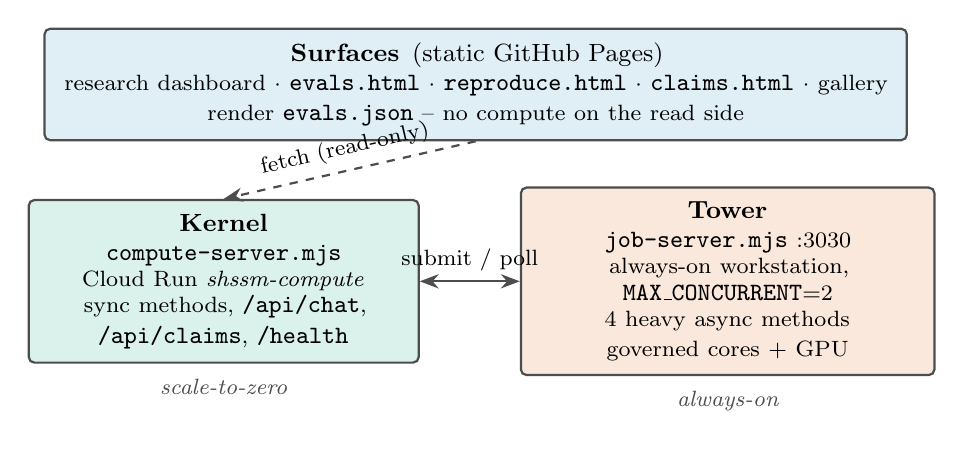
\begin{tikzpicture}[font=\small,
  box/.style={draw=cegrey, thick, rounded corners=2pt, align=center, inner sep=5pt},
  lbl/.style={font=\footnotesize\itshape, text=cegrey},
  flow/.style={-{Stealth[length=2.4mm]}, thick, draw=cegrey}]
  \node[box, fill=ceblue!12, text width=10.6cm] (read) at (0,2.5)
    {\textbf{Surfaces} \,\textnormal{(static GitHub Pages)}\\[1pt]
     \footnotesize research dashboard $\cdot$ \file{evals.html} $\cdot$ \file{reproduce.html} $\cdot$ \file{claims.html} $\cdot$ gallery\\
     \footnotesize render \file{evals.json} -- no compute on the read side};
  \node[box, fill=cegreen!14, text width=4.6cm] (kernel) at (-3.2,0)
    {\textbf{Kernel}\\[1pt]
     \footnotesize \file{compute-server.mjs}\\
     \footnotesize Cloud Run \textit{shssm-compute}\\
     \footnotesize sync methods, \route{/api/chat},\\ \route{/api/claims}, \route{/health}};
  \node[box, fill=ceorange!14, text width=4.9cm] (tower) at (3.2,0)
    {\textbf{Tower}\\[1pt]
     \footnotesize \file{job-server.mjs} :3030\\
     \footnotesize always-on workstation, \code{MAX\_CONCURRENT}=2\\
     \footnotesize 4 heavy async methods\\ \footnotesize governed cores + GPU};
  \node[lbl, below=2pt of kernel] {scale-to-zero};
  \node[lbl, below=2pt of tower] {always-on};
  \draw[flow, dashed] (read.south) -- (kernel.north)
    node[midway, sloped, above, font=\footnotesize] {fetch (read-only)};
  \draw[flow, {Stealth[length=2.4mm]}-{Stealth[length=2.4mm]}] (kernel.east) -- (tower.west)
    node[midway, above, font=\footnotesize] {submit / poll};
\end{tikzpicture}
\caption{The three planes. The read side fetches but never computes; the kernel
serves synchronous methods and submits heavy work to the tower.}
\label{fig:three-planes}
\end{figure}

\subsection{The kernel: synchronous methods on scale-to-zero Cloud Run}
\label{sec:kernel}

The kernel is \file{server/compute-server.mjs}, a zero-dependency Node service that
needs only \code{node:http}, \code{node:https}, \code{node:child\_process} and
\code{node:fs}. It is deployed to Google Cloud Run as the service
\code{shssm-compute} in region \code{asia-south1}; the live release is revision
\code{shssm-compute-00036-llf}, re-confirmed on 2026-06-15 serving a 26-method
registry. A liveness probe reports the running configuration directly:
\route{GET /health} returns
\code{\{ok:true, methods:26, revision:"shssm-compute-00036-llf",
sandbox:"timeout", timeout\_s:90\}}. The same code runs locally on port
\code{3200} for development.

Cloud Run scales the kernel to zero between requests. For a research service whose
traffic is occasional and bursty -- a workbench query here, a chatbot turn there --
this is the right trade: we pay for compute only while a request is in flight, and
a cold start is acceptable latency for an interactive analysis. The cost of that
choice is the request budget. Cloud Run bounds a request at 300\,s and may throttle
CPU outside an active request, so any estimator whose honest runtime is measured in
minutes cannot live on the synchronous path. Those estimators are the tower's
(Section~\ref{sec:tower}); the kernel carries the rest, which return in well under
the timeout.

The kernel's public surface is a small, rate-limited JSON API. CORS is open so the
static read-side pages can fetch it, but those pages only ever read; nothing on the
read side mutates engine state. Table~\ref{tab:kernel-surface} reproduces the
routes. The two model-backed routes, \route{/api/chat} and \route{/api/research},
share a per-instance daily budget and, over cap, return \code{503 daily\_capacity}
with a reset hint rather than a fabricated answer; that budget and its cost ceiling
are treated in Section~\ref{sec:deployment-ops}.

\begin{table}[t]
\centering
\small
\caption{The kernel HTTP surface (\file{server/compute-server.mjs}). Read-side
pages only ever consume these routes; the per-minute and per-day caps are the
abuse and credit guards of Section~\ref{sec:deployment-ops}.}
\label{tab:kernel-surface}
\begin{tabular}{@{}p{3.5cm}l p{7.4cm} l@{}}
\toprule
Route & Method & Purpose & Cap \\
\midrule
\route{/api/compute/run}     & POST & run one registry method on validated params      & 20/min \\
\route{/api/compute/catalog} & GET  & method + dataset registry the workbench binds to  & -- \\
\route{/api/chat}            & POST & AI analyst (Gemini function-calling over registry) & 10/min, 50/day \\
\route{/api/research}        & POST & deep-research assistant (agentic + grounded)       & 5/min, 20/day \\
\route{/api/situate}         & POST & place a result against the verified record         & 30/min \\
\route{/api/claims}          & GET  & epistemic ledger (established / contested / superseded) & -- \\
\route{/api/sri/current}     & GET  & systemic-risk live-feed: latest value              & -- \\
\route{/api/sri/history}     & GET  & systemic-risk live-feed: time series               & -- \\
\route{/api/sri/network}     & GET  & systemic-risk live-feed: directed edges            & -- \\
\route{/api/sri/cron-tick}   & POST & the daily SRI append (Cloud Scheduler only)        & -- \\
\route{/api/event}           & POST & read-side telemetry (aggregate counts, no PII)     & 60/min \\
\route{/health}              & GET  & liveness: methods, revision, sandbox               & -- \\
\route{/metrics}             & GET  & request / cache / rate-limit counters             & -- \\
\bottomrule
\end{tabular}
\end{table}

\subsection{The tower: heavy asynchronous estimators on an always-on workstation}
\label{sec:tower}

Four methods cannot live on the synchronous path, because their honest runtimes
exceed what a scale-to-zero, request-scoped service can carry: \method{ksg\_te}
(exact KSG/Frenzel--Pompe transfer entropy with IAAFT surrogates across all
directed pairs), \method{ksg\_robustness} (its nuisance-grid sweep),
\method{namh\_pipeline} (the end-to-end NAMH estimation, roughly 24 minutes at
$B=200$), and \method{soch\_robustness} (a bootstrap symmetry-test grid). These run
on the tower, \file{server/job-server.mjs}, an always-on service on port
\code{3030} on the group's 22-core workstation, which also carries the GPU used to
offload the transfer-entropy search (treated in the heterogeneous-compute section).

The tower inverts the kernel's request model. \route{POST /api/jobs/submit}
validates the method and returns a \code{job\_<date>\_<hash>} id immediately with
\code{202 Accepted}; the work then runs asynchronously at a small fixed concurrency
(\code{MAX\_CONCURRENT = 2}). A caller polls \route{GET /api/jobs/\{id\}} for the
record, or subscribes to \route{GET /api/jobs/\{id\}/stream}, a Server-Sent-Events
channel that emits \code{progress} events and terminates on \code{done} or
\code{error}. The progress events are exactly the \code{CE\_PROGRESS}-gated lines of
Section~\ref{sec:json-contract}: the tower spawns the same runner with
\code{CE\_PROGRESS=1}, parses each newline-delimited progress object to update the
job, and keeps the final unterminated object as the result.

Job state persists to disk. Every job record is written to \file{.jobs/} as a JSON
file on each transition, so the tower survives a restart: on boot it re-reads
\file{.jobs/}, and any job left \code{running} or \code{queued} is re-queued rather
than lost. Crucially, the tower is also where core governance lives -- it sets a
hard per-job core ceiling and pins the numerical libraries to a single thread each
before spawning R, so two concurrent jobs cannot oversubscribe the machine. That
mechanism, and the 22-core saturation it fixed, are the subject of the
heterogeneous-compute section; here it suffices that the budget is set by the plane
that owns concurrency.

\subsection{The surfaces: render only what is verified}
\label{sec:surfaces}

The third plane is the read side: static GitHub Pages in the sibling
\code{econstellar/} checkout -- the research dashboard, the evaluation and
reproduction pages, the claims panel, the gallery. Nothing on the read side
computes. Each page fetches and renders \file{evals.json}, the single
machine-written artefact of one genuine run of the public evaluation suite, and the
kernel's read-only routes (\route{/api/claims}, the SRI feed). A figure appears on a
surface only because the suite produced it under a pre-registered, failable band; a
regression turns the dashboard red rather than passing silently.

\begin{principle}[Render only what is verified]
\label{prin:render-verified}
The read surfaces display \file{evals.json} and the kernel's read routes; they
execute no analysis of their own. A number reaches a reader only after the
evaluation suite has produced it and checked it against a band fixed before the run.
The read side cannot present an unchecked figure because it cannot compute one.
\end{principle}

This is the architectural counterpart of the catalogue discipline. The kernel will
not run a method that is not registered; the surfaces will not show a result that
the suite has not verified. The separation also keeps the planes honest about cost
and blast radius: the read side is free static hosting that can fail closed, the
kernel pays only while computing, and the heavy machine is reached only through a
job submission that the kernel itself gates.

\subsection{The request lifecycle}
\label{sec:lifecycle}

Every synchronous analysis follows one path, and the path is the same whether the
caller is the workbench, the chatbot, or the test harness. We trace it concretely
for \route{POST /api/compute/run}.

\begin{enumerate}[leftmargin=2em,itemsep=2pt]
\item \textbf{Receive.} The body is read with a 64\,KB cap; an oversized body is
  rejected with \code{413} before parsing, so no request can fan out into unbounded
  memory. A malformed body returns \code{400 bad JSON body}.
\item \textbf{Validate.} \code{validate(method, params)} looks the method up in the
  fixed registry. An unknown name returns \code{400 unknown method}. Each declared
  parameter is then coerced and checked against its typed schema (Section~%
  \ref{sec:registry-guard}); a market name not in the panel's whitelist is rejected
  as \code{unknown series}. What reaches R is a \emph{clean} parameter object, never
  the raw request.
\item \textbf{Route by kind.} If the method is flagged \code{long\_running} it is
  refused here with \code{\{error:"...background job...", async:true\}} and directed
  to the tower; the synchronous endpoint never spawns a heavy estimator.
\item \textbf{Cache.} A 5-minute response cache, keyed on method and cleaned
  parameters, short-circuits repeated identical analyses. Errors are never cached.
\item \textbf{Spawn.} On a cache miss the kernel builds the runner argument vector
  and spawns the registered script under the sandbox (Section~\ref{sec:sandbox}):
  \code{Rscript r/<script>.R '<params-json>'}, wrapped in \code{timeout}. The R
  helper reads exactly the whitelisted dataset and computes.
\item \textbf{Collect.} The child's \code{stdout} is accumulated and parsed as a
  single JSON object (Section~\ref{sec:json-contract}). A \code{124} exit is
  surfaced as an explicit \code{timeout after Ns} error, never a silent hang; a
  non-JSON stdout is reported as such rather than passed through.
\item \textbf{Respond.} The result is wrapped with a provenance stamp -- method
  version, engine revision, cleaned parameters, panel id and byte-hash, timestamp,
  and a permalink that re-runs the exact analysis on load -- and returned.
\end{enumerate}

\begin{figure}[t]
\centering
\resizebox{\textwidth}{!}{%
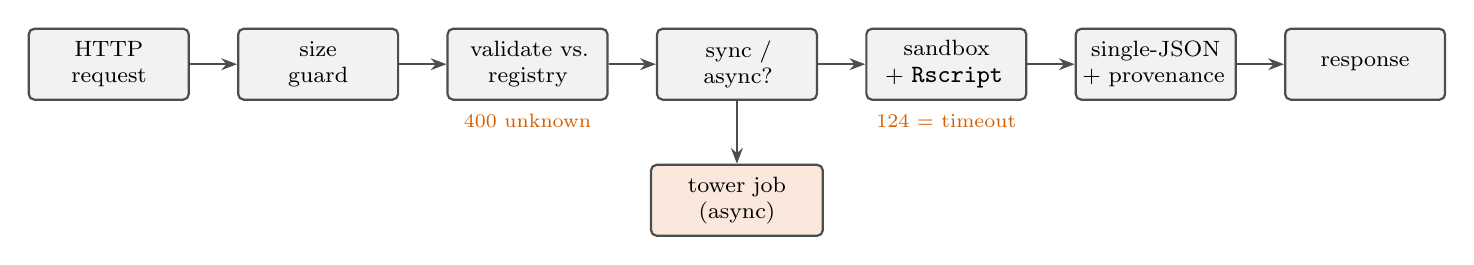
\begin{tikzpicture}[font=\footnotesize, node distance=6mm,
  st/.style={draw=cegrey, thick, rounded corners=2pt, fill=celight, align=center,
    inner sep=4pt, minimum height=9mm, text width=1.75cm},
  ar/.style={-{Stealth[length=2mm]}, thick, draw=cegrey}]
  \node[st] (req) {HTTP\\request};
  \node[st, right=of req] (guard) {size\\guard};
  \node[st, right=of guard] (val) {validate vs.\\registry};
  \node[st, right=of val] (disp) {sync /\\async?};
  \node[st, right=of disp] (spawn) {sandbox\\$+$ \file{Rscript}};
  \node[st, right=of spawn] (json) {single-JSON\\$+$ provenance};
  \node[st, right=of json] (resp) {response};
  \foreach \a/\b in {req/guard, guard/val, val/disp, disp/spawn, spawn/json, json/resp}
    \draw[ar] (\a) -- (\b);
  \node[st, below=8mm of disp, fill=ceorange!14, text width=1.9cm] (tower) {tower job (async)};
  \draw[ar] (disp) -- (tower);
  \node[font=\scriptsize, text=ceorange, below=0.5mm of val.south] {400 unknown};
  \node[font=\scriptsize, text=ceorange, below=0.5mm of spawn.south] {124 $=$ timeout};
\end{tikzpicture}}
\caption{The synchronous request lifecycle. Validation against the registry
precedes any spawn; a method flagged long-running is refused synchronous service
and submitted to the tower; a wall-clock timeout surfaces as an explicit error,
never a silent hang.}
\label{fig:lifecycle}
\end{figure}

Listing~\ref{lst:lifecycle} states the same path as pseudocode, to make the
ordering of the guards unambiguous: validation precedes any spawn, and the registry
lookup is the only thing that turns a request name into an executable.

\begin{lstlisting}[language=JavaScript,caption={The synchronous request path, in
brief. Validation and registry lookup precede every spawn; the runner receives a
cleaned parameter object, never caller-supplied code.},label={lst:lifecycle}]
// POST /api/compute/run  (server/compute-server.mjs)
if (bodyBytes > 64*1024)        return send(413);          // size guard
let payload = JSON.parse(body);                            // 400 on bad JSON
let { method, clean } = validate(payload.method,           // 400 unknown method
                                 payload.params);          // typed-param coercion
if (method.long_running)        return send(400, async);   // -> tower, never here
let hit = cacheGet(method, clean);                         // 5-min TTL
let result = hit
  || await runSandboxed(method, buildArgsJson(method, clean));
return send(200, { ...result,
                   provenance: stamp(method, clean) });    // version+revision+hash
\end{lstlisting}

\subsection{The registry as the primary safety property}
\label{sec:registry-guard}

The central design fact is that the registry is parameterised only. A method entry
is a fixed runner script plus a typed parameter schema -- for example, the
stationarity method binds \code{r/adf.R} with a \code{series} parameter that must be
exactly one market drawn from the panel's whitelist. The runner scripts in
\file{r/} are part of the repository and are never user-supplied. A caller therefore
chooses \emph{which} registered analysis to run and supplies typed inputs to it, but
has no channel through which to inject code, a file path, or a shell fragment.

\begin{invariant}[Parameterised-only execution]
\label{inv:no-rce}
The only executables the engine ever runs are the registered runner scripts shipped
in the repository. A request supplies a method name from a closed registry and a
parameter object validated against that method's typed schema. No request input is
interpreted as code, a path, or a command. There is therefore no
arbitrary-code-execution surface, independent of any sandbox.
\end{invariant}

This is the load-bearing claim, and it is worth being precise about why. The
validation step (Section~\ref{sec:lifecycle}) coerces each parameter to its declared
type and rejects anything outside its domain: series names are checked against the
dataset whitelist, integers and numbers must parse finitely, enumerations must match
a fixed value set, and counts must fall in the method's declared arity. A string that
is not a registered method name does not select a default; it is refused. A probe
such as \code{"DROP\_TABLE; rm -rf /"} as a method name returns \code{400 unknown
method} and reaches no shell. The safety of the public endpoint rests here, on
Invariant~\ref{inv:no-rce}, not on the sandbox.

The sandbox is defence in depth, and we are careful not to overstate it
(Section~\ref{sec:sandbox}). Stating the property in the order it actually holds --
registry first, sandbox second -- matters because the two deployments run different
sandbox modes, and the safety argument must not depend on which one is live.

\subsection{The sandbox, stated precisely}
\label{sec:sandbox}

The runner is launched by one function, \code{runSandboxed}, which detects whether
\code{bwrap} (bubblewrap) is present and adapts.

On the workstation and in local development, where \code{bwrap} is installed, each
analysis runs under bubblewrap with the whole filesystem read-only
(\code{-{}-ro-bind / /}), no network (\code{-{}-unshare-net}, verified to block
outbound), a fresh \code{tmpfs} scratch, and \code{-{}-die-with-parent}, the whole
wrapped in \code{timeout}. The deployed Cloud Run image, by contrast, ships
\emph{without} \code{bwrap}. There the kernel runs in \code{timeout}-only mode --
which is exactly what \route{/health} reports as \code{sandbox:"timeout"} -- and the
isolation boundary is gVisor, the sandbox Cloud Run already places around the
container, together with the read-only image and Cloud Run's own egress posture. We
do \emph{not} claim that \code{bwrap} runs in production; it does not. On Cloud Run,
the kernel boundary is gVisor and a wall-clock timeout bounds each call, while the
no-arbitrary-code guarantee comes from Invariant~\ref{inv:no-rce}, which holds
identically in both modes.

\begin{principle}[Defence in depth, not in place of the registry]
\label{prin:depth}
The sandbox narrows what a misbehaving runner could touch; it is not the reason the
public endpoint is safe to expose. That reason is the parameterised-only registry.
Where \code{bwrap} is present we additionally pin the filesystem read-only and the
network off; where it is not, gVisor and a per-call timeout provide the kernel
boundary. The safety claim is invariant to which mode is live.
\end{principle}

Either way, one method call is bounded by \code{COMPUTE\_TIMEOUT\_S} -- 90\,s in the
deployed image, default 60\,s -- and a timeout is surfaced as an explicit error, so
a pathological input degrades to a clean \code{timeout after Ns}, never an unbounded
run.

\subsection{The JSON contract and the purity of stdout}
\label{sec:json-contract}

The data contract is deliberately minimal: one JSON object in, one JSON object out.
A request carries \code{\{method, params\}}; a runner prints exactly one JSON object
to \code{stdout} and exits. This single discipline is what lets a method run
identically across the three planes -- the cloud container, the workstation, and the
harness all spawn the same script and parse the same object. The R helpers in
\file{r/\_io.R} centralise emission through one function, \code{ce\_emit}, which
serialises the result and quits; failures emit \code{\{error: ...\}} through
\code{ce\_fail}.

The fragility this guards against is real. R routinely writes to \code{stdout} for
reasons unrelated to the result -- a warning that a KPSS p-value lies beyond the
tabulated range, a package's registration notice on load. Any such stray line would
be concatenated with the JSON and break the parse. The helpers therefore set
\code{options(warn = -1)} and suppress load messages, so that the only thing on
\code{stdout} is the result object.

Progress reporting is the interesting case, because the heavy tower estimators
genuinely need to stream progress, yet the kernel's stdout must stay pure. The
engine resolves this with a single environment gate. The helper \code{ce\_progress}
emits a newline-terminated progress line \emph{only} when the async worker has set
\code{CE\_PROGRESS=1}; under the synchronous kernel that variable is unset, so
\code{ce\_progress} is a silent no-op and the pure-single-JSON contract of
\route{/api/compute/run} is unchanged. The tower (Section~\ref{sec:tower}) sets
\code{CE\_PROGRESS=1}, reads the newline-delimited progress lines to drive its
event stream, and treats the final unterminated object as the result. The same
runner thus serves both planes without a branch in its own logic.

\subsection{The data plane}
\label{sec:data-plane}

The primary stored panel is \file{papers/contagion-channels/data/G20.xlsx}: daily
equity log-returns for 18 markets spanning 2006-01-12 to 2026-03-18, which yields
$18 \times 17 = 306$ directed market pairs for the information-flow methods. Transfer
entropy is computed on log-returns, which are $I(0)$, never on price levels, which
are $I(1)$; the stationarity gate is enforced rather than assumed. A second panel,
\code{g20\_24}, supplies the 24-series set used by the NAMH methods (19 equity
indices plus five commodity futures), read from the published \code{namh} package's
bundled data so that the cloud image and the workstation see byte-identical inputs.

Both panels are byte-hashed with SHA-256 at kernel and tower startup, and the hash
travels with the result in its provenance stamp. A reported figure therefore names
the exact data state it was computed against, which is what makes a later
reproduction meaningful: the panel is identified not by a filename but by the hash
of its bytes. Datasets that are planned but not provisioned -- an intraday G20 panel,
for instance -- are present in the registry as honest placeholders with no series
list, so \code{validate} refuses any analysis against them rather than fabricating a
result. This is the data-plane expression of the same discipline that governs the
method catalogue: a capability is exposed only when it is real.
}{}
\IfFileExists{sections/03-substrate-methods.tex}{\section{The methodological substrate and the method registry}
\label{sec:substrate}

The engine's claim to be a single substrate, rather than a bag of scripts, rests on
one observation. The six published frameworks it carries (NAMH, SOCH,
contagion-channels, WaveQTE, the commodity study, and MCPFM) do not each need a
private toolchain. They are recombinations of a small number of estimator-level
operations: measure how a series remembers its own past, split its variance across
time scales, quantify directed information flow, build a null by surrogate
construction, partition a network into communities, decompose a system's
connectedness, attribute a transmitted shock to a structural channel, and validate
a binary call against a curve. We call these the \emph{eight primitives}. Every one
of the \textbf{26} registry methods is one or more primitives wired to a dataset,
and every method ships with a pre-registered, failable test of its own output. The
registered voice is deliberate: we would rather have twenty-six checked methods than
fifty asserted ones.

This section names the eight primitives and their mathematical objects
(\S\ref{sec:primitives}), shows how the registry's six families map onto them
(\S\ref{sec:registry}), then gives the transfer-entropy estimator in full because it
is the load-bearing one and the only quantity the GPU path must reproduce bit-for-bit
(\S\ref{sec:ksg}). We close with the determinism discipline that makes the estimators
reproducible (\S\ref{sec:determinism}) and the failable-test rule that governs
catalogue entry (\S\ref{sec:failable}).

\begin{figure}[t]
\centering
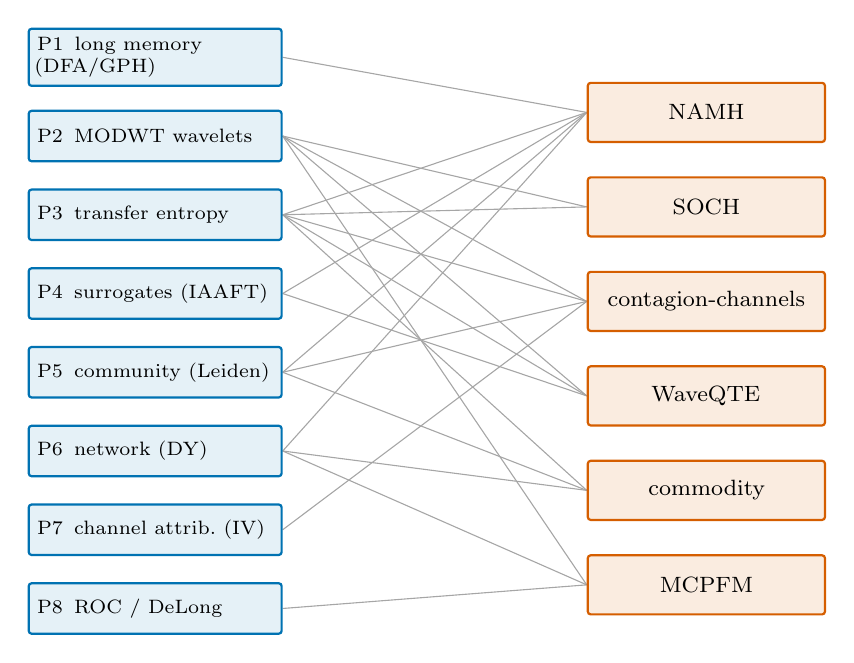
\begin{tikzpicture}[
  prim/.style={draw=ceblue, thick, fill=ceblue!10, rounded corners=1pt, align=left,
    inner sep=3pt, text width=3.0cm, font=\scriptsize, minimum height=6.4mm},
  fw/.style={draw=ceorange, thick, fill=ceorange!12, rounded corners=1pt, align=center,
    inner sep=3pt, text width=2.8cm, font=\footnotesize, minimum height=7.5mm},
  edge/.style={draw=cegrey!50, line width=0.4pt}]
  \node[prim] (P1) at (0,7.0) {P1\, long memory (DFA/GPH)};
  \node[prim] (P2) at (0,6.0) {P2\, MODWT wavelets};
  \node[prim] (P3) at (0,5.0) {P3\, transfer entropy};
  \node[prim] (P4) at (0,4.0) {P4\, surrogates (IAAFT)};
  \node[prim] (P5) at (0,3.0) {P5\, community (Leiden)};
  \node[prim] (P6) at (0,2.0) {P6\, network (DY)};
  \node[prim] (P7) at (0,1.0) {P7\, channel attrib.\ (IV)};
  \node[prim] (P8) at (0,0.0) {P8\, ROC / DeLong};
  \node[fw] (NAMH) at (7.0,6.3) {NAMH};
  \node[fw] (SOCH) at (7.0,5.1) {SOCH};
  \node[fw] (CC)   at (7.0,3.9) {contagion-channels};
  \node[fw] (WQ)   at (7.0,2.7) {WaveQTE};
  \node[fw] (CM)   at (7.0,1.5) {commodity};
  \node[fw] (MC)   at (7.0,0.3) {MCPFM};
  \begin{scope}[on background layer]
    \foreach \p in {P1,P3,P4,P5,P6} \draw[edge] (\p.east) -- (NAMH.west);
    \foreach \p in {P2,P3}          \draw[edge] (\p.east) -- (SOCH.west);
    \foreach \p in {P2,P3,P5,P7}    \draw[edge] (\p.east) -- (CC.west);
    \foreach \p in {P2,P3,P4}       \draw[edge] (\p.east) -- (WQ.west);
    \foreach \p in {P3,P5,P6}       \draw[edge] (\p.east) -- (CM.west);
    \foreach \p in {P2,P6,P8}       \draw[edge] (\p.east) -- (MC.west);
  \end{scope}
\end{tikzpicture}
\caption{The substrate carries the programme. Each published framework (right,
in orange) composes a subset of the eight estimator-level primitives (left, in
blue); the same transfer-entropy and network machinery recurs across elements.
The composition shown is the principal-primitive view; Section~\ref{sec:elements}
gives each element in full.}
\label{fig:substrate}
\end{figure}

\subsection{The eight primitives}
\label{sec:primitives}

Table~\ref{tab:primitives} names each primitive, the mathematical object it returns,
its canonical reference, and the registry methods that instantiate it. The primitives
are estimator-level, not framework-level: a single method (for example
\method{namh\_pipeline}) composes several, and a single primitive (for example P3) is
shared across frameworks that otherwise have nothing in common.

\begin{table}[t]
\centering
\footnotesize
\caption{The eight-primitive substrate. Each primitive is an estimator-level
operation with a fixed mathematical object and a canonical reference; the registry
methods in the last column instantiate it on a whitelisted dataset.}
\label{tab:primitives}
\begin{tabular}{@{}p{2.25cm}p{4.5cm}p{2.7cm}p{4.55cm}@{}}
\toprule
\textbf{Primitive} & \textbf{Object computed} & \textbf{Reference} & \textbf{Example methods} \\
\midrule
P1 long-memory &
  Hurst exponent $H$; $\phi(H)=1-2|H-\tfrac12|$ &
  DFA / GPH / Qu &
  \method{dfa\_hurst}, \method{namh\_hurst} \\
P2 multi-scale &
  MODWT detail variance $\{\sigma^2_{d_j}\}$ &
  \cite{barunik2018} &
  \method{wavelet}, \method{wavelet\_coherence} \\
P3 information flow &
  directed TE $T_{Y\to X}$ &
  \cite{schreiber2000,kraskov2004,frenzel2007} &
  \method{ksg\_te}, \method{namh\_te}, \method{wqte} \\
P4 surrogate null &
  IAAFT / permutation null distribution &
  \cite{schreiber1996} &
  \method{ksg\_te}, \method{namh\_pipeline} \\
P5 community &
  partition / modularity $Q$ &
  \cite{traag2019} &
  \method{network}, \method{namh\_pipeline} \\
P6 connectedness &
  GFEVD spillover; frequency bands &
  \cite{diebold2012,diebold2014,barunik2018} &
  \method{connectedness}, \method{spillover\_rolling} \\
P7 channel attribution &
  per-channel share via IV / 2SLS &
  \cite{bhandari2026contagion} &
  \method{channel\_attribution} \\
P8 ROC validation &
  AUC; DeLong / Hansen test &
  \cite{bhandari2025mcpfm} &
  MCPFM out-of-sample call \\
\bottomrule
\end{tabular}
\end{table}

\paragraph{P1 -- long memory.}
The object is the Hurst exponent $H$, the scaling exponent of detrended fluctuation
analysis. On the cumulative profile $y_t=\sum_{s\le t}(x_s-\bar x)$ the series is cut
into log-spaced boxes, each box is detrended by a local polynomial, the
root-mean-square residual fluctuation $F(n)$ is taken per box length $n$, and $H$ is
the slope of $\log F(n)$ on $\log n$. The transparent realisation
(\file{r/dfa\_hurst.R}) implements this directly; the published path
(\file{r/namh\_hurst.R}) calls \method{namh::estimate\_hurst\_panel}
\citep{namhpkg} on a rolling window and supplies the NAMH node weight
$\phi(H)=1-2|H-\tfrac12|$, a local-efficiency score peaking at the random-walk value
$H=\tfrac12$. We read $H$ on log-returns, which are $I(0)$, never on price levels,
which are $I(1)$.

\paragraph{P2 -- multi-scale decomposition.}
The object is the variance of a series across dyadic time scales, obtained from the
maximal-overlap discrete wavelet transform (MODWT). Boundary-affected coefficients
are removed by the \method{brick.wall} operator before the per-scale variance
$\sigma^2_{d_j}$ is read, so scale $d_1$ corresponds to roughly $2$--$4$ day
fluctuations, $d_2$ to $4$--$8$ days, and so on (\file{r/wavelet.R}). The same
decomposition underlies the scale-resolved squared coherence
$\rho^2_j=\mathrm{cor}(d^x_j,d^y_j)^2$ (\file{r/wavelet\_coherence.R}), which we label
honestly as a discrete scale-resolved coherence rather than the continuous Morlet
time-frequency object. P2 is the Stage-1 primitive of NAMH, MCPFM, and the
contagion-channels frameworks.

\paragraph{P3 -- directed information flow.}
The object is transfer entropy $T_{Y\to X}$, the reduction in uncertainty about
$X_{t+1}$ from knowing the past of $Y$ beyond the past of $X$ \citep{schreiber2000}.
Three estimators sit under this primitive: the engine's own
Kraskov--St{\"o}gbauer--Grassberger / Frenzel--Pompe $k$-nearest-neighbour estimator
(\method{ksg\_te}, derived in full in \S\ref{sec:ksg}); the published \method{namh}
package's Euclidean RANN variant (\method{namh\_te}); and a transparent
wavelet-quantile measure built from MODWT and quantile regression (\method{wqte}).
These are different estimators of the same object and their magnitudes are not
cross-comparable, a boundary the runners state explicitly.

\paragraph{P4 -- surrogate construction.}
The object is a null distribution for a dependence statistic, built without parametric
assumptions. The engine's default is the iterative amplitude-adjusted Fourier
transform (IAAFT) of \citet{schreiber1996}: a surrogate of the source series is formed
by alternately imposing the source's Fourier amplitude spectrum and its empirical
amplitude distribution until the rank order stabilises, so the surrogate preserves the
source's linear autocorrelation and marginal while destroying its (possibly nonlinear)
predictive dependence on the target. Significance of a directed TE edge is then
$p=(1+\#\{T^{\text{surr}}\ge T^{\text{obs}}\})/(B+1)$. Surrogate subtraction also
defines \emph{effective} transfer entropy (\S\ref{sec:ksg}).

\paragraph{P5 -- community detection.}
The object is a partition of a directed weighted network into communities, with a
modularity score $Q$. The published NAMH pipeline uses the Leiden algorithm
\citep{traag2019}, which guarantees well-connected communities and corrects the
resolution-limit pathologies of Louvain; the transparent \method{network} surface uses
a Walktrap partition on the undirected projection of a Granger graph. A community
result is only as meaningful as the adjacency it partitions: when the upstream FDR
gate retains no edges, the partition is degenerate by construction and is reported as
such, not dressed up.

\paragraph{P6 -- connectedness and network formation.}
The object is a system's total and directional connectedness from a vector
autoregression's generalised forecast-error variance decomposition (GFEVD). The
time-domain index is Diebold--Y{\i}lmaz \citep{diebold2012,diebold2014}; the
frequency decomposition is Barun{\'i}k--K{\v r}ehl{\'i}k \citep{barunik2018}, which
splits the total connectedness index across short ($\le 5$ day), medium ($5$--$20$
day), and long ($>20$ day) bands by partitioning the spectral GFEVD at
$\omega=2\pi/P$ (\file{r/connectedness.R}). The rolling variant
(\method{spillover\_rolling}) tracks the index through time.

\paragraph{P7 -- structural channel attribution.}
The object is the share of a transmitted shock attributable to each of a fixed set of
economic channels, identified with instruments rather than read off a reduced-form
correlation. The published contagion-channels pipeline
\citep{bhandari2026contagion,ccpkg} runs a two-stage detection-and-attribution
procedure: Stage 1 detects directed tail linkages, Stage 2 attributes them to five
mutually exclusive channels (trade, financial, geopolitical, behavioural, monetary)
by instrumental-variables / two-stage least squares (\file{r/channel\_attribution.R}).
This is the primitive that turns a network edge into an economic explanation.

\paragraph{P8 -- ROC validation.}
The object is the area under the receiver-operating-characteristic curve (AUC) of a
binary forecast, with a significance test on the AUC. This is the primitive by which a
predictive claim is held to account out of sample; MCPFM \citep{bhandari2025mcpfm}
reports AUC with a DeLong test in version 1 and, under a pre-registered
re-evaluation, a Hansen superior-predictive-ability test in version 2. We report both
openly (\S\ref{sec:failable}).

\subsection{The registry and its six families}
\label{sec:registry}

The \textbf{26} methods are grouped into six families by the statistical question they
answer, not by which primitives they happen to share; a family is the unit a reader
reasons about, while a primitive is the unit the code reuses. Table~\ref{tab:families}
gives the family structure with a representative method or two from each, its
primitive composition, and one verified value. The complete per-method registry with
every pre-registered acceptance band is Appendix~A; here we show only the shape.

\begin{table}[t]
\centering
\footnotesize
\caption{The six families of the registry (26 methods total), with a representative
method per family, the substrate primitives it composes, and one verified value. The
full per-method acceptance bands are in Appendix~A. Counts: stationarity 5, volatility
5, information flow 5, connectedness 6, contagion 2, reproduction 3.}
\label{tab:families}
\begin{tabular}{@{}p{4.2cm}p{3.8cm}p{1.5cm}p{4.7cm}@{}}
\toprule
\textbf{Family ($n$)} & \textbf{Representative method} & \textbf{Primitives} & \textbf{Verified value} \\
\midrule
Stationarity, cointegration, panels (5) &
  \method{panel\_unit\_root}, \method{vecm} & -- &
  IPS $-77.26$; Johansen rank 3 \\
Volatility, long memory, spectra (5) &
  \method{dfa\_hurst}, \method{wavelet} & P1, P2 &
  India $H=0.542$; $d_1=47.07\%$ \\
Information flow (5) &
  \method{ksg\_te}, \method{wqte} & P3, P4 &
  USA$\to$Japan TE $0.154234$ \\
Connectedness, networks (6) &
  \method{connectedness}, \method{network} & P5, P6 &
  TCI $30.25\%$; density $0.5667$ \\
Contagion, systemic risk (2) &
  \method{channel\_attribution}, \method{sri\_daily} & P5, P7 &
  GFC trade $27.9\%$ \\
Reproduction, formal verification (3) &
  \method{namh\_reproduce}, \method{soch\_robustness} & P1--P5 &
  $\max|\Delta|\,1.55\times10^{-15}$ \\
\bottomrule
\end{tabular}
\end{table}

Two points the table cannot show. First, the families are not silos: the same
estimator can appear in several. Transfer entropy (P3) is the engine of the
information-flow family, but it is also the first stage of the NAMH pipeline in the
reproduction family. Second, a method may be either a \emph{transparent} realisation
built from substrate parts, or a \emph{published} method that calls a paper's own
package directly. \method{wqte} reimplements the WaveQTE Stage-1 primitive from
\method{waveslim} and \method{quantreg} because the packaged estimator does not load
in the image; \method{soch\_profile}, \method{channel\_attribution},
\method{namh\_hurst}, and \method{namh\_te} call \method{sochcontagion}, \method{contagionchannels},
and \method{namh} respectively, so the live engine runs the paper's own code. The
distinction is recorded on every such method, because a transparent reimplementation
and a bit-exact package call carry different reproduction claims.

\subsection{The transfer-entropy estimator in full}
\label{sec:ksg}

Transfer entropy is the load-bearing primitive: it is the most-used edge statistic in
the programme, the one quantity the GPU path must reproduce bit-for-bit, and the one
whose estimator subtleties most repay a careful statement. We give it here at the
depth of the implementation in \file{r/\_ksg\_core.R} and \file{gpu/ksg\_gpu.py}.

\paragraph{Transfer entropy as conditional mutual information.}
For an ordered pair $(Y\to X)$ with history length (lag) $\ell$, transfer entropy is
the conditional mutual information between the one-step future of the target and the
past of the source, given the past of the target \citep{schreiber2000}:
\begin{equation}
\label{eq:te-cmi}
T_{Y\to X} \;=\; I\!\left(X_{t+1}\,;\, Y_t^{(\ell)} \;\middle|\; X_t^{(\ell)}\right),
\qquad
Y_t^{(\ell)} = \bigl(Y_t, Y_{t-1}, \dots, Y_{t-\ell+1}\bigr).
\end{equation}
The conditioning set $Z = X_t^{(\ell)}$ is the target's own past; the marginal blocks
are $X = X_{t+1}$ (the future, dimension $1$) and $Y = Y_t^{(\ell)}$ (the source past,
dimension $\ell$). The engine's default is $\ell=1$ (\method{ksg\_te} parameter
\code{lag}), the Markov-1 conditioning under which the past blocks collapse to the
single lagged values $X_t$ and $Y_t$. The embedding aligns the future $X_{t+1}$ with
the lag blocks ending at $t$, so that one point of the joint sample is
$(X_{t+1}, Y_t^{(\ell)}, X_t^{(\ell)})$.

\paragraph{The KSG / Frenzel--Pompe estimator.}
Rather than bin the joint density, the estimator counts neighbours. Following
\citet{kraskov2004} for mutual information and \citet{frenzel2007} for its conditional
extension, the conditional mutual information in Eq.~\eqref{eq:te-cmi} is estimated by
\begin{equation}
\label{eq:ksg-cmi}
\widehat{I}(X;Y\mid Z) \;=\; \psi(k)
  \;+\; \frac{1}{N}\sum_{i=1}^{N}\Bigl[\,
    \psi\!\bigl(n^Z_i+1\bigr) - \psi\!\bigl(n^{XZ}_i+1\bigr) - \psi\!\bigl(n^{YZ}_i+1\bigr)
  \,\Bigr],
\end{equation}
where $\psi$ is the digamma function, $k$ is the neighbour count (parameter \code{k},
default $4$), and $N$ is the number of embedded points. The three counts are taken in
the marginal sub-spaces of the conditioning set and its unions with each variable:
$n^Z_i$, $n^{XZ}_i$, $n^{YZ}_i$ count the points whose distance from point $i$ in the
$Z$, $(X,Z)$, and $(Y,Z)$ sub-spaces respectively is strictly less than $\epsilon_i$.
This is the \method{.ksg\_cmi} function; the transfer entropy
$T_{Y\to X}=\widehat{I}$ at $Z=X_t^{(\ell)}$ is \method{.te}.

\paragraph{The max-norm and the neighbour radius.}
The metric is the maximum (Chebyshev) norm,
\begin{equation}
\label{eq:maxnorm}
\Norm{u-v}_\infty \;=\; \max_{c} \,\lvert u_c - v_c \rvert,
\end{equation}
taken over all coordinates of the relevant space. The radius $\epsilon_i$ is the
max-norm distance from point $i$ to its $k$-th nearest neighbour in the \emph{full}
joint space $(X,Y,Z)$, self excluded. The engine works in raw return coordinates and
does not standardise, because the G20 series are already daily log-returns and the
max-norm is not scale-invariant, so a $z$-score would change the estimate; the runners
and the GPU helper both note this. Computing $\epsilon_i$ exactly under the max-norm on
a tree built for the Euclidean norm uses the inclusion $\Norm{\cdot}_\infty \le
\Norm{\cdot}_2 \le \sqrt{d}\,\Norm{\cdot}_\infty$: an inflated $L_2$ candidate list is
pulled, exact Chebyshev distances are recomputed, the $k$-th smallest is taken, and a
point's radius is accepted only once its candidate list provably covers that radius
(\method{.maxnorm\_knn\_dist}). This makes the radius exact, not approximate.

\paragraph{The one-dimensional count boundary.}
A subtlety the bit-exactness gate caught, and which a careful reader should know about,
lives in how the strict-inequality counts are realised. For a sub-space of dimension
$\ge 2$ the count is taken directly as $\#\{j\neq i : \Norm{u_i-u_j}_\infty <
\epsilon_i\}$ by recomputing the max-norm and applying $<$ (\method{.count\_kd}). For a
one-dimensional sub-space (which arises for the $Z$ count when $\ell=1$) the engine
uses a sorted-array realisation via \method{findInterval}
(\method{.count\_1d}), testing membership against the half-open interval
$[v-\epsilon,\, v+\epsilon)$ rather than the absolute form $|v_j-v|<\epsilon$. The two
disagree on exactly one floating-point boundary tie: when $|v_j-v|$ rounds to exactly
$\epsilon$ but $v-\epsilon$ rounds down, the interval form \emph{includes} the point
that the absolute form rejects. The engine's choice is the \method{.count\_1d}
convention, and the GPU helper reproduces that convention host-side rather than the
textbook absolute form (\file{gpu/ksg\_gpu.py}, \method{\_count\_1d\_engine\_batch}),
so the observed estimate matches the engine's own six-decimal emission exactly. The
lesson, recorded as a learning, is to gate on the estimator's own output including its
floating-point boundary conventions, not on the textbook formula.

\paragraph{Effective transfer entropy.}
The raw estimate of Eq.~\eqref{eq:ksg-cmi} carries a finite-sample bias that does not
vanish under the null of no information flow. Following the surrogate bias-correction
of \citet{marschinski2002}, the \emph{effective} transfer entropy subtracts the mean of
the estimator over surrogate source series that share the source's marginal and linear
autocorrelation but carry no directed dependence on the target:
\begin{equation}
\label{eq:ete}
T^{\text{eff}}_{Y\to X}
  \;=\; T_{Y\to X} \;-\; \frac{1}{B}\sum_{b=1}^{B} T_{\,\tilde Y^{(b)}\to X},
\qquad \tilde Y^{(b)} \sim \text{IAAFT}(Y),
\end{equation}
with $B$ surrogates drawn by the IAAFT of \S\ref{sec:primitives}. The same surrogate
ensemble gives the permutation $p$-value $p=(1+\#\{T_{\tilde Y\to X}\ge
T_{Y\to X}\})/(B+1)$. The published NAMH pipeline computes
Eq.~\eqref{eq:ete} explicitly (\method{TE\_eff} in \file{r/namh\_pipeline.R}); the
deterministic \method{namh\_te} method returns the raw estimate only and states that
the effective TE and the $p$-values, being surrogate-dependent and unseeded in the
package, are not bit-reproducible and belong to the async pipeline.

\paragraph{GPU equivalence on the observed estimate.}
The cost is an $O(N^2)$ max-norm neighbour search, once per directed pair and once per
surrogate, which previously saturated the workstation. The search now runs on the
RTX 3000 Ada GPU through two \method{numba.cuda} kernels (one for the radii, one for
the three counts), with the IAAFT surrogates batched on the host
(\file{gpu/ksg\_gpu.py}). Crucially, the \emph{observed} transfer entropy is the only
quantity the evaluation suite gates, and it is held bit-exact to the CPU estimator:
the measured maximum discrepancy is $7\times10^{-16}$ and the six-decimal emission is
identical, across $\ell\in\{1,2\}$ and $k\in\{4,5\}$, verified by
\file{gpu/equiv\_gate.R}. The $p$-value is an unseeded surrogate draw in both the CPU
and GPU paths and is never claimed reproducible. Defaulting to the GPU therefore can
never move a published number; a box with no CUDA device, or a forced \code{CE\_GPU=0},
degrades silently to the governed CPU path.

\subsection{Determinism and reproducibility of the estimators}
\label{sec:determinism}

Reproducibility of a Monte-Carlo estimator requires that two facts be pinned: the
random stream, and the order of reduction. The engine pins both.

\paragraph{The random stream.}
Where a method's result depends on a draw, the runner sets
\code{RNGkind("L'Ecuyer-CMRG")} and \code{set.seed(42)} before the computation. The
combined multiple-recursive generator of \citet{lecuyer1999} is chosen because it
splits into independent sub-streams that \method{parallel::mclapply} can hand to its
fork workers deterministically: under a fixed seed each child stream derives
reproducibly from the master seed. The canonical surrogate count is $B=200$. The
published NAMH end-to-end run is the clearest case (\file{r/namh\_pipeline.R}): the
\method{namh} package's own IAAFT generator is unseeded, so the paper's published
surrogate run is not bit-reproducible; the engine's runner pins the seed and the
generator so that its result \emph{is} reproducible for a fixed
$\{\text{seed}, n_{\text{cores}}\}$ pair. That dependence on the core count, through
the stream split, is stated rather than hidden. The two \method{ksg} methods are
deliberately \emph{not} seeded, so their surrogate $p$-values are an honest
non-reproducible draw in both the CPU and GPU paths; their reproducible content is the
observed TE, which carries no randomness.

\paragraph{The order-free reduction.}
The directed-pair and grid loops are order-free: the result is a set of per-pair
estimates reduced by operations (sums, means, rank correlations, set overlaps) that do
not depend on the order in which the pairs complete. This is what lets the worker
count be governed without touching a number. The shared helper
\method{ce\_ncores} in \file{r/\_io.R} sets the \method{mclapply} budget from a base of
\code{detectCores()} minus a reserve, overridden by an explicit \code{n\_cores}, and
clamped last by a hard ceiling \code{CE\_MAX\_CORES} (which the tower sets to
$\lfloor(\text{cpus}-2)/\text{MAX\_CONCURRENT}\rfloor=10$ on the workstation). BLAS
threading is pinned to one thread per spawn. Because the loops are order-free, changing
the worker count from one to ten never changes a TE value; it only governs CPU. This is
the formal content of an invariant the system depends on.

\begin{invariant}[Worker-count neutrality]
\label{inv:order-free}
For every method that reduces a set of independently computed per-pair or per-grid
estimates, the emitted result is invariant to the number of parallel workers and to the
order in which they complete. Core governance and BLAS pinning therefore change CPU
occupancy, never a published value.
\end{invariant}

\subsection{A failable test per method}
\label{sec:failable}

The discipline that makes the registry trustworthy is one rule, applied without
exception.

\begin{principle}[Catalogue entry requires a failable test]
\label{prin:failable}
A method enters the registry only with a pre-registered, failable acceptance band on
its own output, fixed before the run. A regression turns the public dashboard red
rather than passing silently; a hole is marked, never filled; and the band is never
edited to fit a result.
\end{principle}

Three verified examples show the principle at work, drawn from
Table~\ref{tab:families} and the registry. They are stated with their provenance, in
the registered measured voice, because a real number with a band is worth more than an
adjective.

\begin{cexample}[An observed estimate in band]
\label{ex:ksg}
The \method{ksg\_te} method on the 18-market G20 panel returns the USA$\to$Japan
transfer entropy as $\mathbf{0.154234}$, across $306$ directed pairs of which $108$ are
significant at $p<0.05$ against IAAFT source surrogates. The pre-registered band is
$T\in[0.150,0.158]$; the value sits inside it. The same observed estimate is the
quantity the GPU path reproduces to $7\times10^{-16}$, and a full-panel re-run of all
$306$ pairs reproduced $0.154234$ exactly.
\end{cexample}

\begin{cexample}[A stability claim across nuisance parameters]
\label{ex:robustness}
The \method{ksg\_robustness} sweep re-runs the same estimator across the grid
$k\in\{3,4,6,8\}\times\ell\in\{1,2\}$ and checks two pre-registered conditions: that the
headline directed edge is ranked first at every grid point, and that the mean Spearman
rank correlation of the full directed-TE vector against the baseline lies in
$[0.6,0.85]$. Both hold: the mean Spearman is $\mathbf{0.7282}$ (minimum $0.581$), and
USA$\to$Japan is the \#1 directed edge across all eight $(k,\ell)$ settings. The
headline link is therefore robust to the estimator's nuisance parameters, not an
artefact of one choice.
\end{cexample}

\begin{cexample}[A published estimate held to a tight band]
\label{ex:namh}
The \method{namh\_hurst} method, running the published \method{namh} package on its
rolling-window panel, returns a mean Hurst exponent for Gold of $\mathbf{0.490}$
($0.4899$). The pre-registered band is $[0.4889,0.4909]$, a tight window that would
fail loudly on any drift in the package or the data. The value is reproduced to
$\max|\Delta|\,1.55\times10^{-15}$ same-machine by the \method{namh\_reproduce}
$\Delta$-verifier.
\end{cexample}

Honest negatives are themselves results under Principle~\ref{prin:failable} and are
immutable facts of the record, not failures to be hidden. The MCPFM out-of-sample call
returns AUC $0.581$ (DeLong $p=0.030$) in version 1; a pre-registered version-2
re-evaluation returns AUC $0.470$ (Hansen SPA $p=0.031$), and that lower figure is
reported openly with a reproduce status of honest-pending. The NAMH pipeline's own
Benjamini--Hochberg FDR gate retains $0/552$ directed edges at the canonical
configuration, so its masked network, fixed point, and communities are degenerate by
construction and are emitted as measured, in the dashboard's honest amber, rather than
magnitude-dressed. A method that asserted a clean network there would be the failure;
reporting the empty gate is the discipline.
}{}
\IfFileExists{sections/04-heterogeneous.tex}{\section{Heterogeneous compute: core governance, GPU offload, and the asynchronous tower}
\label{sec:heterogeneous}

The methods in the substrate are not uniform in cost. Most return in well under a
second on a stored panel; a few -- the transfer-entropy estimators in particular --
spend their time in an $O(n^2)$ nearest-neighbour search and, run carelessly, can
saturate a workstation. This section describes how \engine{} runs that uneven load
safely. There are three concerns and one rule that ties them together. The rule is
that \emph{the number of workers must never change a number}: every heavy loop in the
engine is an order-free reduction over independent directed pairs or grid cells, so
how we split the work governs only the use of the machine, never the result. Given
that rule, the three concerns are how many CPU cores a job may use (core governance),
whether the heaviest primitive can be moved off the CPU entirely (GPU offload), and
how a job that runs for minutes rather than milliseconds is managed without blocking
the synchronous kernel (the asynchronous tower).

\subsection{Core governance: one budget, wired everywhere}
\label{sec:core-governance}

The motivating failure is concrete and was diagnosed to a single line. Three methods
-- \method{ksg\_te}, \method{ksg\_robustness}, and \method{sri\_daily} -- each
hard-coded their worker count as \code{ncores <- detectCores() - 1L}. On the
22-logical-core workstation that is $21$ \code{mclapply} workers per job, and it
ignored the job's own \code{n\_cores} request entirely. With the tower configured to
run two jobs at once and the numeric libraries left multi-threaded, two concurrent
\method{ksg\_robustness} jobs forked $2 \times 21 = 42$ worker processes, each of
which could in turn spawn its own BLAS threads on top of the fork. That multiplicative
oversubscription pinned all $22$ cores at $100\%$ and hung the machine; the reboot
left two \method{ksg\_robustness} records stranded in the \code{running} state. The
fault was not the estimator but the absence of a single place that decides how many
cores a job may use.

The fix is exactly that single place. In \file{r/\_io.R} we added one governed
budget, \method{ce\_ncores}$(p,\ \mathit{reserve})$, and wired it into all six
\code{mclapply} call sites. Its precedence is fixed and the ceiling is clamped last:

\begin{lstlisting}[language=R,caption={The single core budget (\file{r/\_io.R}).},label=lst:ce-ncores]
ce_ncores <- function(p = NULL, reserve = 2L) {
  b <- max(1L, parallel::detectCores() - as.integer(reserve))      # 1. base
  if (!is.null(p) && !is.null(p$n_cores)) {                        # 2. job override
    req <- suppressWarnings(as.integer(p$n_cores))
    if (!is.na(req) && req >= 1L) b <- req
  }
  cap <- suppressWarnings(as.integer(Sys.getenv("CE_MAX_CORES", "")))
  if (!is.na(cap) && cap >= 1L) b <- min(b, cap)                   # 3. HARD ceiling, last
  max(1L, b)
}
\end{lstlisting}

A base of \code{detectCores() - reserve} can be raised or lowered by an explicit
\code{n\_cores} parameter, but the environment ceiling \code{CE\_MAX\_CORES} is applied
afterwards and cannot be exceeded by any caller. The function always returns at least
one. The complementary half lives in the tower process manager. The job server in
\file{server/job-server.mjs} sets, for every R subprocess it spawns,
\[
  \texttt{CE\_MAX\_CORES} \;=\; \Big\lfloor \tfrac{\texttt{cpus}-2}{\texttt{MAX\_CONCURRENT}} \Big\rfloor,
\]
which evaluates to \textbf{10} on the 22-core workstation (reserving two threads for
the operating system and the Node server). Because the ceiling is divided by the
concurrency level, $\texttt{MAX\_CONCURRENT}$ jobs cannot jointly oversubscribe the
box: two concurrent jobs now use at most $20$ cores, never $42$, and a job that asks
for $21$ under a ceiling of $10$ is forced down to $10$. The same spawn pins each
numeric library to a single thread (\code{OPENBLAS\_NUM\_THREADS},
\code{OMP\_NUM\_THREADS}, \code{MKL\_NUM\_THREADS}, \code{VECLIB\_MAXIMUM\_THREADS},
\code{NUMEXPR\_NUM\_THREADS} all set to \code{1}), removing the second factor of the
oversubscription. The resulting budget is surfaced in the tower's \route{/health}
response and startup log as \code{core\_budget}, so the governing number is observable
rather than implicit.

Pinning the BLAS threads is not only a safety measure. A multi-threaded BLAS reduces
in a non-deterministic order, so summation results can differ in their last bits from
run to run; pinning each library to one thread fixes that order and makes the numeric
result reproducible. The core-governance change therefore buys a reproducibility gain
on top of the safety one, and it does so without any risk to the published numbers,
because of the order-free structure of the loops it governs.

\begin{invariant}[Worker count does not change a result]
\label{inv:worker-count}
Every loop governed by \method{ce\_ncores} is a reduction over independent units --
directed pairs for the transfer-entropy methods, $(k,\text{lag})$ cells for the
robustness grid -- whose combination (a set of per-pair records, a mean, a ranking)
does not depend on the order in which the units are evaluated or on how they are
split across workers. Capping the worker count, or pinning BLAS to one thread,
therefore changes only CPU occupancy and floating-point reduction order, never the
estimate the eval suite gates.
\end{invariant}

\subsection{GPU offload of the transfer-entropy search}
\label{sec:gpu-offload}

Core governance makes the CPU path safe; the GPU path removes the heaviest load from
the CPU altogether. The hot primitive is the Kraskov--St{\"o}gbauer--Grassberger
estimator in its Frenzel--Pompe conditional-mutual-information form
\citep{kraskov2004,frenzel2007,schreiber2000}: for each point we find $\epsilon_i$,
the max-norm distance to its $k$-th neighbour in the joint
$(\text{dst}_{t+1},\,\text{src}_t,\,\text{dst}_t)$ space, then count neighbours with
marginal max-norm distance strictly less than $\epsilon_i$ in three sub-spaces. That
search is $O(n^2)$ and is exactly the work that hung the workstation. We ported it to
two \code{numba.cuda} kernels (CUDA $12.4$, numba $0.63.1$ \citep{lam2015numba}) and
run it on an NVIDIA RTX 3000 Ada Laptop GPU (compute capability $8.9$, $8$\,GB). One
thread handles one $(\text{search},\text{point})$ pair, so a directed pair's observed
estimate and all of its surrogates run in a single launch, amortising the launch and
host--device transfer overhead. The kernels compute in FP64.

The choice of FP64 over FP32 is deliberate and is the crux of why a faster device does
not threaten the engine's discipline. The Ada GPU's FP32 path is faster still, but the
KSG estimate is the anchor that the eval suite checks; an approximate value would move
that anchor and break the gate. We therefore pay for double precision so that the GPU
result is not close to the CPU result but \emph{identical} to it. Max-norm distances
are computed by absolute value, subtraction, and maximum, all exact IEEE operations,
so the $k$-th order statistic of an identical multiset and the strict-$<$ integer
counts are the same on host and device.

That identity is enforced by a failable gate, \file{gpu/equiv\_gate.R}, which runs the
GPU helper and the engine's own CPU estimator on a small bounded case and exits
non-zero unless they agree. The observed maximum absolute difference is at most
$7\times 10^{-16}$ -- it was $6.7\times 10^{-16}$ in the NAMH re-estimation -- and the
six-decimal emitted values are bit-for-bit identical. The gate caught a subtle and
instructive discrepancy. The engine's one-dimensional neighbour count, used for the
conditioning sub-space at $\text{lag}=1$, tests membership with
\code{findInterval(v - eps)} rather than the absolute form $|dp - v| < \epsilon$. On
the rare boundary tie where $|dp - v|$ rounds to exactly $\epsilon$ but $v - \epsilon$
rounds down, the interval form \emph{includes} a point that the absolute form excludes.
The GPU helper replicates the engine's interval form host-side for that
one-dimensional case, so the published estimate (the eval anchor) is preserved exactly
rather than merely approximately. The lesson is that when a published estimator is
ported to a faster device, the gate must be the estimator's own output, including its
floating-point boundary quirks, not the textbook formula.

\begin{principle}[Gate on the estimator's output, not its textbook form]
\label{prin:gate-output}
The only quantity the eval suite gates from the transfer-entropy methods is the
observed TE (the \method{ksg\_te} band and the \method{ksg\_robustness} rankings and
Spearman correlations). Because the GPU reproduces that quantity bit-for-bit, GPU
execution can be the default without ever moving a published number. The significance
$p$-value is a different matter: it comes from IAAFT surrogates
\citep{schreiber1996}, and the engine seeds neither transfer-entropy method, so the
$p$-value is a non-reproducible draw on the CPU path and on the GPU path alike. We
never claim it reproducible, and the gate never tests it.
\end{principle}

Dispatch and fallback are handled by \method{ce\_ksg\_gpu\_pairs} in
\file{r/\_ksg\_core.R}, shared by \method{ksg\_te} and \method{ksg\_robustness}. The
default is \code{AUTO}: setting \code{CE\_GPU=0} forces the CPU path, otherwise the
dispatcher probes for a usable CUDA device, and if one is present it writes the
returns matrix as a raw column-major binary alongside a JSON spec
($n$, $k$, lag, surrogate count, the pair list), invokes \file{gpu/ksg\_gpu.py}, and
parses the per-pair results, stamping a \code{compute\_path} field. Robustness is the
point of the design: any failure at all -- \code{CE\_GPU=0}, no CUDA device, a missing
or broken helper, a malformed or short result -- returns \code{NULL}, and the caller
then runs its governed CPU \code{mclapply} path. A box with no GPU, or one with a
broken toolkit, degrades silently and safely to the path that core governance already
made safe.

\begin{figure}[t]
\centering
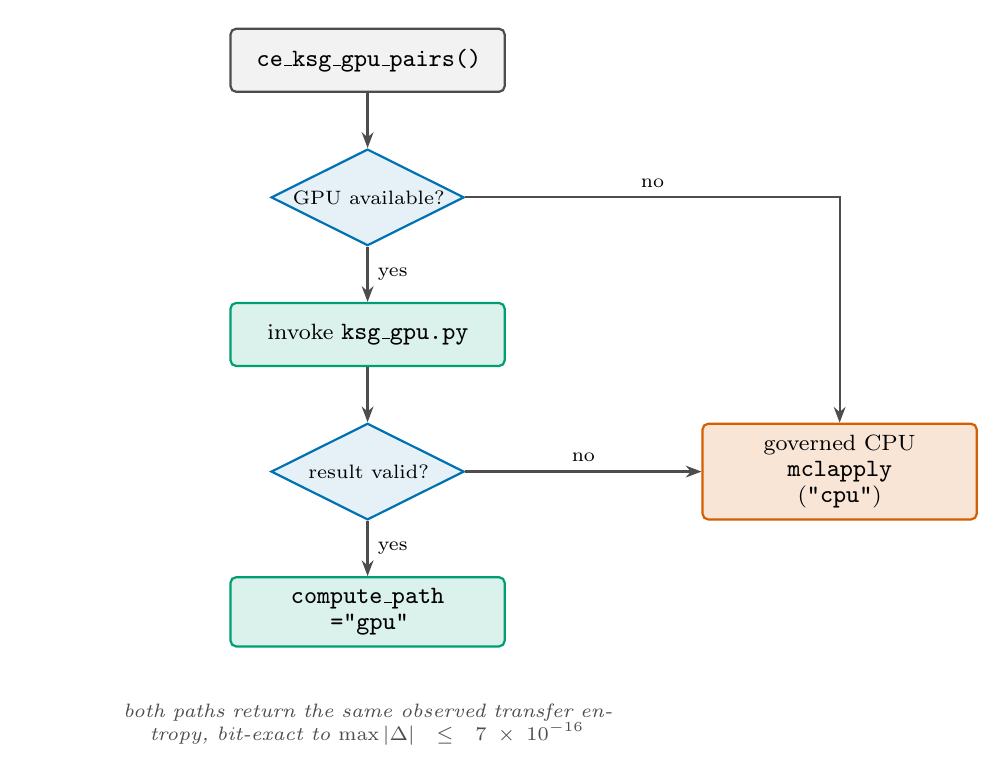
\begin{tikzpicture}[font=\footnotesize,
  bx/.style={draw=cegrey, thick, rounded corners=2pt, fill=celight, align=center,
    inner sep=4pt, text width=3.2cm, minimum height=8mm},
  gpu/.style={bx, fill=cegreen!14, draw=cegreen},
  cpu/.style={bx, fill=ceorange!16, draw=ceorange},
  dec/.style={draw=ceblue, thick, fill=ceblue!10, diamond, aspect=2, align=center,
    inner sep=1pt, font=\scriptsize, text width=1.9cm},
  ar/.style={-{Stealth[length=2mm]}, thick, draw=cegrey}]
  \node[bx] (entry) {\code{ce\_ksg\_gpu\_pairs()}};
  \node[dec, below=7mm of entry] (d1) {GPU available?};
  \node[gpu, below=7mm of d1] (inv) {invoke \file{ksg\_gpu.py}};
  \node[dec, below=7mm of inv] (d2) {result valid?};
  \node[gpu, below=7mm of d2] (ok) {\code{compute\_path}\\\code{="gpu"}};
  \node[cpu, right=30mm of d2] (cpu) {governed CPU\\\code{mclapply}\\(\code{"cpu"})};
  \draw[ar] (entry) -- (d1);
  \draw[ar] (d1) -- node[right,font=\scriptsize]{yes} (inv);
  \draw[ar] (inv) -- (d2);
  \draw[ar] (d2) -- node[right,font=\scriptsize]{yes} (ok);
  \draw[ar] (d1.east) -| node[near start,above,font=\scriptsize]{no} (cpu.north);
  \draw[ar] (d2.east) -- node[above,font=\scriptsize]{no} (cpu.west);
  \node[align=center, font=\scriptsize\itshape, text=cegrey, below=6mm of ok,
    text width=8.4cm] (note) {both paths return the same observed transfer entropy,
    bit-exact to $\max|\Delta| \le 7\times10^{-16}$};
\end{tikzpicture}
\caption{GPU dispatch with governed-CPU fallback. ``GPU available?'' tests
\code{CE\_GPU}$\neq$0, a present CUDA device, and a successful probe; any failure,
including a malformed result, falls back to the path that core governance already
made safe. The offload changes only where the observed transfer entropy is
computed, never its value.}
\label{fig:dispatch}
\end{figure}

The surrogate inner loop stays on the host. IAAFT is dominated by a per-surrogate FFT
rather than by the neighbour search, so the helper runs it batched over surrogates
with a batched FFT and feeds the resulting source series into the same two kernels.
The measured effect of the offload is twofold -- it is faster and it frees the CPU. On
this workstation, $12$ directed pairs with $B=99$ surrogates run in $82$ seconds at
roughly one core on the GPU against $289$ seconds across roughly seven cores on the
governed CPU, a \textbf{3.5$\times$} speed-up that also returns six cores to other
work. In the isolated trial on a deterministic coupled system the kernel search alone
runs up to \textbf{73.76$\times$} faster ($n=3000$), and between $32\times$ and
$74\times$ faster across $n \in \{2000, 3000, 5000\}$, all bit-exact. The
confirmation that matters is the full-panel re-run: the exact workload that hung the
machine -- the full G20 panel, $306$ directed pairs at $B=99$ -- completed on the GPU
in \textbf{35.6 minutes} at $100\%$ of \emph{one} core with a peak of $388$\,MB of
host memory, returning $106$ of $306$ pairs significant and the USA${\to}$Japan
estimate at $\mathbf{0.154234}$, identical to the CPU value. The saturation that hung
the 22-core box is gone, and the heaviest, most parallel primitive in the engine now
runs on the device best suited to it.

\subsection{The asynchronous tower}
\label{sec:async-tower}

A run that takes thirty-five minutes does not belong on the synchronous kernel, which
runs scale-to-zero on Cloud Run under a request timeout. Four methods are heavy enough
to need a different home: \method{ksg\_te}, \method{ksg\_robustness},
\method{namh\_pipeline}, and \method{soch\_robustness}, each flagged
\code{long\_running} in the registry. These run on the always-on workstation tower
managed by \file{server/job-server.mjs}, which executes the same parameterised-only R
registry as the kernel -- it discovers methods from \file{r/*.R} and refuses anything
else -- but asynchronously. A \route{POST /api/jobs/submit} validates the workspace
and the method name, returns a \code{job\_id} immediately, and queues the work; the
manager runs at most \code{MAX\_CONCURRENT} jobs at a time under the core budget of
Section~\ref{sec:core-governance}. Each job record and its result persist to a
\file{.jobs/} directory on disk and are reloaded on startup, so a job survives a
restart and is addressable by a permalink for thirty days; a job left
\code{running} by a crash is requeued rather than lost.

Progress is reported without compromising the engine's output contract. The kernel
requires that a method's standard output be a single pure JSON object, so progress
lines cannot simply be printed. The progress emitter \method{ce\_progress} in
\file{r/\_io.R} is therefore silent unless the environment variable \code{CE\_PROGRESS}
is set, and only the tower sets it:

\begin{lstlisting}[language=R,caption={Progress is opt-in, so the synchronous contract is never polluted (\file{r/\_io.R}).},label=lst:ce-progress]
ce_progress <- function(fraction = NA, stage = "", elapsed_s = NA) {
  if (!nzchar(Sys.getenv("CE_PROGRESS"))) return(invisible(NULL))   # silent under the kernel
  cat(toJSON(list(`__progress__` = TRUE, fraction = fraction,
                  stage = stage, elapsed_s = elapsed_s),
             auto_unbox = TRUE, na = "null"), "\n", sep = "")
  flush(stdout())
}
\end{lstlisting}

Under the synchronous kernel this is a no-op and the stdout remains a single JSON
object. Under the tower, which spawns each method with \code{CE\_PROGRESS=1}, the
method emits newline-terminated progress objects tagged \code{\_\_progress\_\_}; the
job manager parses those lines, updates the job record, and pushes them to any
subscriber over Server-Sent Events at \route{/api/jobs/:id/stream}, while the final
unterminated JSON object is read as the result. The same heavy method thus serves two
callers -- a synchronous one that sees only the answer and an asynchronous one that
sees the answer and the progress -- from one code path, with the environment, not the
source, deciding which behaviour is in force.
}{}
\IfFileExists{sections/05-ai-layer.tex}{\section{The AI layer: a natural-language client, not a privileged path}
\label{sec:ai-layer}

The engine is reachable in plain language. A researcher can ask a question -- ``is the
UK equity series stationary?'', ``which market sends the most information to Japan?''
-- and receive an answer that ran the real econometrics rather than a plausible
paragraph. Two routes provide this. \route{/api/chat} is a fast analyst backed by
Gemini 2.5 Flash; \route{/api/research} is a deeper assistant backed by Gemini 2.5 Pro
that both runs analyses and grounds its synthesis in literature. The design problem
they pose is not capability but containment: a language model that can trigger compute
is a new way to reach the engine, and we must be sure it is not a new way to reach
anything else. The whole of this section is organised around the claim that it is not,
because the AI layer is a client of the engine on exactly the same footing as a script
or a web form, with no execution surface of its own.

\subsection{The chat route}
\label{sec:chat-route}

\route{/api/chat} is a single function-calling turn followed by a summary. The user's
message goes to Gemini with one tool, \method{run\_analysis}, whose parameters are a
method name and its typed arguments; the model either answers conceptually with no tool
call or emits exactly one call. That call is not executed as written. It is passed
through the same \method{validate} routine every other caller uses -- which rejects an
unknown method or a mistyped parameter -- and only the validated, cleaned method and
arguments reach \method{runSandboxed}. The result is then handed back to the model for
a second turn that explains the numbers in prose. The route returns
\code{\{reply, ran\}}, where \code{ran} records the method, the cleaned parameters, the
raw result, and the wall time, so the natural-language answer is always accompanied by
the machine record it was built from. The system prompt is a careful econometrician,
not a generic assistant; in particular it carries the stationarity rule discussed
below, so the model never reports a price level as stationary.

\subsection{The research route}
\label{sec:research-route}

\route{/api/research} is the same idea at publication depth, and it runs in two phases.
Phase~A is an agentic loop, bounded to a few steps, in which Gemini 2.5 Pro is given
the \method{run\_analysis} tool and runs live econometrics wherever the question admits
it -- it may issue several calls, see their results, and call again, each call passing
through the same \method{validate} and \method{runSandboxed} path as the chat route.
Phase~B is a grounded synthesis: the analyses executed in Phase~A are summarised into a
digest, the digest and the question are sent back to the model with a
\code{google\_search} tool, and the model writes the final answer grounded in real
sources. The route returns
\[
  \texttt{\{answer,\ citations[],\ searches[],\ analyses[],\ steps\}},
\]
so the caller receives the prose answer, the grounding citations (title and URI), the
search queries the model issued, the full record of every analysis it ran, and the
step count. The citations are read from the model's grounding metadata, not invented by
the prose.

The two phases are kept separate for a concrete reason of API behaviour rather than
preference. Function-calling and \code{google\_search} grounding are not reliably
combined within one Gemini request, so the engine does not attempt to. Instead it runs
the tools in their own passes and carries the executed analyses forward as text into
the grounded pass; the model still cites real literature \emph{and} reasons over real
live numbers, but the two tool modes never share a single request. This is the kind of
fragility a systems report should name: the separation is a workaround for a model-API
constraint, documented in the route itself.

The system prompt for the research route does substantial work, and all of it is fact,
not flourish. It injects the eight-primitive substrate -- long-memory estimation,
MODWT wavelet decomposition, transfer entropy, surrogate inference, community
detection, network-formation game theory, structural attribution, and classifier
validation -- so the model reasons in the engine's own vocabulary; it names the
frameworks those primitives instantiate; and it injects the verified-results table
verbatim with the instruction to quote it exactly and never alter it, so a number the
model states is a number the engine has checked. It also carries the stationarity rule
as an inviolable constraint.

\begin{principle}[The stationarity rule]
\label{prin:stationarity}
Transfer entropy and the other dependence measures are estimated on $I(0)$ log-returns,
never on $I(1)$ price levels. Equity price levels carry a unit root (a random walk with
drift); log-returns, $\mathrm{diff}(\log \text{price})$, are typically stationary. The
stored G20 panel is already log-returns, so any ``stationary'' verdict over it concerns
returns, and the model is required to say so explicitly (``UK equity \emph{returns} are
stationary'', not ``the UK market is stationary''). Embedding this rule in the prompt
prevents the most common and most consequential error an unguided model would make on
financial series.
\end{principle}

\subsection{The safety argument}
\label{sec:ai-safety}

The reason the AI layer can be exposed at all is that it adds no power. Everything it
can cause to happen, a direct caller of \route{/api/compute/run} could already cause to
happen; everything a direct caller cannot do, the AI layer cannot do either. This is
worth stating precisely, because it is the load-bearing claim of the whole design.

\begin{invariant}[The AI layer is a client, not a privileged path]
\label{inv:ai-client}
The model cannot execute arbitrary code. It can only name a method already in the
registry and supply typed parameters for it, and it can only read that method's
returned result. Its proposed call is validated by the same \method{validate} routine
and executed by the same \method{runSandboxed} path as any other request, so it
inherits every guard those impose and introduces no new execution surface. The
registry of parameterised methods is the boundary; the language model sits outside it,
on the same side as a script or a browser.
\end{invariant}

This follows directly from the implementation. A function call from Gemini is data: a
method string and an arguments object. It is subjected to \method{validate} before it
is allowed to mean anything, and \method{validate} is the same gate the public compute
route uses, so an attempt to name a method that does not exist, or to pass a parameter
of the wrong type or shape, is rejected before any R process is spawned. There is no
path by which the model can supply code, a file path, a shell fragment, or a network
target; the parameterised-only registry that is the engine's primary guard against
arbitrary execution applies to the model exactly as it applies to everyone else. The
AI layer widens the engine's audience -- it makes the methods reachable by people who
would not write the JSON by hand -- without widening its attack surface.

\subsection{Rate limits and the cost bound}
\label{sec:ai-cost}

Because each model turn costs real money, the AI routes are bounded on several axes, and
the bound that matters most is a hard ceiling on spend rather than a courtesy throttle.
The per-IP limiter caps \route{/api/research} at roughly five requests per minute and
roughly twenty per day, with \route{/api/chat} held to a higher but still bounded rate;
these stop a single client from monopolising the service or slowly draining the credit.
Above those sits the ceiling that bounds the worst case regardless of how many clients
attack at once. Each instance permits at most $400$ paid LLM turns per UTC day, and
Cloud Run is configured for at most two instances, so the fleet-wide maximum is
\[
  400 \ \text{turns/instance/day} \times 2 \ \text{instances}
  \;=\; \textbf{at most 800 paid turns/day}.
\]
The day counter resets at UTC midnight, and when the cap is reached the routes return a
service-unavailable response with a retry hint rather than paying for another turn. The
limiter is process-local and resets on restart, which is acceptable precisely because
the per-instance daily cap multiplied by the instance ceiling already gives a bounded
fleet-wide daily maximum: the AI layer cannot, under any traffic pattern, spend more
than that.
}{}
\IfFileExists{sections/06-verification.tex}{\section{Verification and Epistemics}
\label{sec:verification}

The engine's claim to trustworthiness does not rest on the authors' assurance.
It rests on a small set of machine-run artefacts that any reader can inspect and,
given the repository, re-execute: a pre-registered evaluation suite that grades
live computation against failable numerical bands, a nightly loop that re-runs
that suite and writes its own findings into a ledger it does not get to edit by
hand, a claims record that demotes rather than deletes, and a thin formal layer
in which one identity is closed in a proof assistant with an honest count of what
remains open. This section describes those four artefacts and the single property
that ties them together: the apparatus is built so that its own correctness, and
the wiring that enforces it, are themselves things that can fail a test in public.

\subsection{The evaluation suite}
\label{sec:verification-evals}

The suite lives in \file{evals/run-evals.mjs} and emits a single artefact,
\file{evals.json}. Each catalogue method has exactly one row. A row names the
method, the parameter object it is called with, an \code{expected} string stating
the pre-registered band in plain language, a \code{source} citing where that band
comes from, and a \code{check} function that extracts one quantity from the live
result and returns a boolean. The runner posts the request to the deployed engine
(or, for the four heavy asynchronous methods, submits a real job to the
workstation job server and polls it to completion), applies the check, and records
the verdict. It computes; it does not read a cached number. The most recent full
run recorded \textbf{26 of 26 rows passing} (0 fail, 0 pending) against the live
service.

Three rules govern the artefact, and each is enforced by construction rather than
by convention.

\begin{principle}[Bands are pre-registered and failable]
A band is fixed before the run, from a documented verified value, and is written
so that the result can fall outside it. Where a method's verified tuple does not
pin a full configuration, the band degrades to an invariant check that can still
fail on the wrong shape, a non-finite value, an unstable system, or a wrong
verdict, never to a check that always passes.
\end{principle}

\begin{principle}[The artefact is never hand-edited]
\file{evals.json} is the output of one genuine execution of the committed runner.
A red row is information, not a defect to be quietly corrected in the file. To
change a number one re-runs the suite, not the artefact.
\end{principle}

\begin{principle}[A band failure halts; only extraction may be calibrated]
Failures split in two. A \emph{band} failure means the engine is wrong: work
stops and the cause is investigated. An \emph{extraction} failure means the
harness misread the result's shape: the check is corrected and the whole suite is
re-run. Fixing extraction is calibration, not gaming, only when the expected band
is left untouched.
\end{principle}

The bands are not decorative, and several of them encode a number whose value is
the point. Three rows make the discipline concrete. The first is an ordinary
positive result. The synchronous transfer-entropy row \method{ksg\_te} calls the
estimator on the USA and Japan series and checks the directed edge:

\begin{lstlisting}[language=JavaScript]
{ m: "ksg_te", p: { series: ["USA", "Japan"] }, async: true,
  expected: "USA->Japan full-sample KSG TE in [0.150,0.158] (verified 0.1542)",
  src: "A2 + #39 anchor",
  check: r => { const e = (r.edges || r.pairs || [])
      .find(x => /usa/i.test(x.from) && /japan/i.test(x.to)) || {};
    const v = num(e.te ?? e.TE);
    return { value: v, pass: inBand(v, 0.150, 0.158) }; } }
\end{lstlisting}

\noindent The last full run returned $0.154234$ for this edge, inside the band,
from a real job on the tower (\code{job\_20260612\_92fa3f31}); the worked trace in
Section~\ref{sec:worked} follows that exact call from HTTP request to single-JSON
response. The second is a degenerate negative that must \emph{stay} degenerate.
The \method{namh\_pipeline} row runs the full NAMH surrogate pipeline end to end
under a fixed seed and checks that, under the paper's own Benjamini--Hochberg
gate \citep{benjamini1995}, the network is empty:

\begin{lstlisting}[language=JavaScript]
{ m: "namh_pipeline",
  p: { n_surrogates: 200, window_index: 1, seed: 42, n_cores: 2 }, async: true,
  expected: "FDR retains 0/552 under the paper's own gate (degenerate, honest amber);
             raw te_mean in [-0.2242,-0.2222]",
  check: r => { const w = (r.per_window || [])[0] || {}; const f = w.fdr || {};
    const c = r.config || {};
    return { value: num(w.te_raw && w.te_raw.mean),
      pass: num(f.n_edges) === 0 && num(f.n_possible) === 552
            && w.degenerate === true
            && inBand(num(w.te_raw && w.te_raw.mean), -0.2242, -0.2222)
            && c.seed === 42 && c.rng === "L'Ecuyer-CMRG" }; } }
\end{lstlisting}

\noindent Here a \emph{populated} network would be the failure and the empty one
is the pass: the row insists on \textbf{0 of 552} directed edges retained in the
window, the window flagged \code{degenerate}, the raw window mean inside
$[-0.2242,-0.2222]$ (the last run returned $-0.22322165$), and the generator
pinned to L'Ecuyer's combined multiple-recursive scheme \citep{lecuyer1999} at
seed 42. The third is the live systemic-risk index. The \method{sri\_daily} row
recomputes the static-panel index in full from the stored panel and checks it
against a band one part in $10^{5}$ wide, $[0.00848, 0.00850]$, around the first
honest point $0.00849$ over 306 directed pairs. A reproduction target this tight
can only be met by re-running the same computation, which is the property the row
exists to certify.

The suite is honest about its own operational hazards, which is itself part of
the discipline. The runner rides out a Cloud Run cold start with a second,
longer health probe, because a single short probe once misreported a live engine
as unreachable while all rows passed; it waits politely under the engine's
rate limit rather than recording a self-inflicted red; and asynchronous rows are
either real tower jobs with persistent identifiers or honest \code{async\_pending}
placeholders, never fabricated values. The artefact records, per row, the
measured value, the elapsed milliseconds, whether the engine served it from cache,
and any job identifier, so that the run can be audited line by line.

\subsection{The nightly self-learning loop}
\label{sec:verification-loop}

The suite would be a static check were it not re-run. The centrepiece of the
verification layer is the loop in \file{scripts/nightly-loop.sh}, installed under
\code{cron} at \code{10 7 * * *} UTC, fifty minutes after the 06:00 UTC systemic-
risk tick. Its design intent is to survive a reboot, to be loud in the cron log
when something regresses, and never to silently repair a problem it should
surface. The cron entry and the script are installed and self-tested; at the time
of writing the loop has not yet completed an unattended run, so its cadence is
reported as configured rather than demonstrated. It re-arms the long-lived job
server only if its port is closed, killing
nothing, then runs the six steps summarised in Table~\ref{tab:loop} and pictured
in Figure~\ref{fig:loop}.

\begin{figure}[t]
\centering
\resizebox{\textwidth}{!}{%
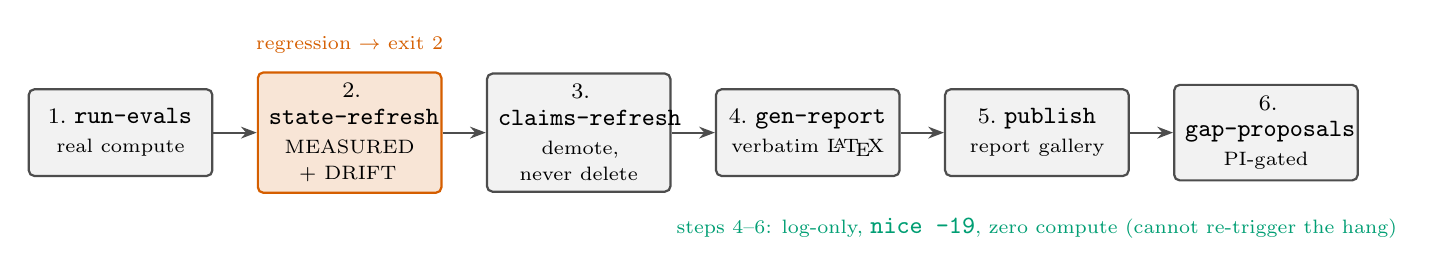
\begin{tikzpicture}[font=\footnotesize, node distance=5.5mm,
  st/.style={draw=cegrey, thick, rounded corners=2pt, fill=celight, align=center,
    inner sep=4pt, text width=2.05cm, minimum height=11mm},
  gate/.style={st, fill=ceorange!16, draw=ceorange},
  ar/.style={-{Stealth[length=2mm]}, thick, draw=cegrey}]
  \node[st]              (s1) {1.\ \code{run-evals}\\[1pt]\scriptsize real compute};
  \node[gate, right=of s1] (s2) {2.\ \code{state-refresh}\\[1pt]\scriptsize MEASURED $+$ DRIFT};
  \node[st, right=of s2] (s3) {3.\ \code{claims-refresh}\\[1pt]\scriptsize demote, never delete};
  \node[st, right=of s3] (s4) {4.\ \code{gen-report}\\[1pt]\scriptsize verbatim \LaTeX};
  \node[st, right=of s4] (s5) {5.\ \code{publish}\\[1pt]\scriptsize report gallery};
  \node[st, right=of s5] (s6) {6.\ \code{gap-proposals}\\[1pt]\scriptsize PI-gated};
  \foreach \a/\b in {s1/s2,s2/s3,s3/s4,s4/s5,s5/s6} \draw[ar] (\a)--(\b);
  \node[font=\scriptsize, text=ceorange, above=1mm of s2] {regression $\to$ exit 2};
  \node[font=\scriptsize, text=cegreen, below=4mm of s5.south]
    {steps 4--6: log-only, \code{nice -19}, zero compute (cannot re-trigger the hang)};
\end{tikzpicture}}
\caption{The six-step nightly loop. Step~2 governs the exit code, turning a
regression into a non-zero exit and a red dashboard; steps 4--6 do no computation,
so the reporting layer can never re-trigger a saturation. No step deletes a claim
or edits a result.}
\label{fig:loop}
\end{figure}

\begin{table}[t]
\centering
\small
\begin{tabular}{@{}c l p{0.62\textwidth}@{}}
\toprule
Step & Script & What it does, and how it stays honest \\
\midrule
1 & \file{run-evals.mjs} & Re-arms the job server (port-guarded, no kills), then runs the full suite, async rows as real tower jobs, writing a fresh \file{evals.json}. \\
2 & \file{state-refresh.mjs} & Measures live health, the eval summary, and the SRI feed; rewrites \emph{only} the \code{MEASURED} block of \file{STATE.md} and appends a dated \code{DRIFT} line on any regression. Its exit code is the loop's: non-zero means a problem line was written. \\
3 & \file{claims-refresh.mjs} & Re-verifies the mapped claims against the same night's artefact: a pass bumps \code{last\_verified}; a red marks the claim \code{contested} and inserts the other side of the pair. Never deletes. Log-only, so a database outage cannot repaint the night. \\
4 & \file{gen-compute-report.mjs} & Renders a LaTeX run report verbatim from \file{evals.json}; never recomputes, never invents, renders failures as loudly as passes. Run \code{nice -n 19} so it always yields to a tower job. \\
5 & \file{publish-reports.mjs} & Copies each report PDF and a thumbnail into the static report gallery and rewrites its manifest. Pure file copy, \code{nice}'d, non-fatal. \\
6 & \file{gap-proposals.mjs} & Mines the demand signals the engine exposes, applies the pre-registered rule, and emits PI-review candidate skeletons. Never auto-deploys. \\
\bottomrule
\end{tabular}
\caption{The six steps of \file{scripts/nightly-loop.sh}. Step~2 owns the loop's
exit code, so a regression is loud in the cron log; steps 4--6 are log-only and
non-fatal, so a rendering or reporting fault cannot mask the canary in steps
1--3.}
\label{tab:loop}
\end{table}

Two properties of the loop are worth drawing out. The first is the division of
authority between its steps. The eval suite and \method{state-refresh} are the
canary: \method{state-refresh} exits 2 on any regression -- the engine
unreachable, a failed eval, a changed method count, or a systemic-risk feed stale
beyond three weekdays -- and that exit code becomes the loop's, so a problem is
never silent. Everything downstream is deliberately log-only and non-fatal. A
BigQuery outage in the claims step, a LaTeX fault in the report step, or a missing
checkout in the publish step is recorded and skipped; none is allowed to repaint
a night whose real signal is the suite and the state ledger above it. The report
step is the one that can always yield, which is why it runs \code{nice -n 19}: it
is pure rendering plus a single \code{pdflatex} pass, and it must never contend
with a long-running tower job for the processor.

The second property is the one we hold to most firmly: the loop's own wiring is a
failable eval. A separate test, \file{evals/loop-integrity.test.mjs}, asserts
that the steps exist, that the artefact paths the steps pass to one another agree,
that the set of claims the refresher maps is a subset of the suite's rows, that no
step on the nightly path issues a delete, that the gap rule and its PI gate are
intact, and that the installed state is reported honestly. We record this as an
invariant because it is the load-bearing one.

\begin{invariant}[The verifier verifies itself]
\label{inv:self}
The self-checking loop is subject to the same standard as the methods it checks:
its wiring -- step existence, artefact-path agreement, the claims-to-evals
subset relation, the no-delete rule, and the pre-registered, PI-gated gap rule
-- is itself a pre-registered, failable test. The apparatus that asserts
correctness can therefore fail loudly when its own assumptions break.
\end{invariant}

\noindent That this is not a formality is visible in the test's history: its first
execution was red, eleven of twenty, and all of the failures were the harness
misreading shapes (a \code{m:} key written \code{method:}, a quoted path, a
\code{DELETE} appearing inside a comment). Those were extraction failures,
calibrated per the band-versus-harness rule with the bands untouched, and the
test then went green -- exactly the discipline the suite imposes on every other
row, now imposed on the loop itself.

\subsection{The learning ledger}
\label{sec:verification-ledger}

The engine keeps a single state file, \file{STATE.md}, with three blocks. The
\code{MEASURED} block is machine-written by \method{state-refresh} and is never
touched by hand; the \code{LEDGER} block is appended by working sessions; the
\code{LEARNING} block stages each burned lesson through a fixed lifecycle --
\emph{fail} (the lesson enters when something breaks), \emph{investigate} (the
cause is named), \emph{verify} (the fix is proven), and \emph{distill} (the lesson
is promoted to a consultable Skill). Thirteen learnings are recorded;
Table~\ref{tab:learnings} states each in a line.

\begin{table}[t]
\centering
\footnotesize
\begin{tabular}{@{}c l l p{0.50\textwidth}@{}}
\toprule
ID & Date & Stage & Lesson (terse) \\
\midrule
L1 & 2026-06-11 & distilled & A robustness grid must anchor through the paper's own scripts and estimation universe before any badge is written. \\
L2 & 2026-06-11 & distilled & Moving the engine root silently changes API-key resolution and can ship a chat-disabled revision; check the WARN line. \\
L3 & 2026-06-10 & distilled & Yahoo serves \code{close: null} for hours after a session; the finite-close guard makes the tick skip honestly. The schedule is the guard. \\
L4 & 2026-06-11 & distilled & Eval failures split into band failures (stop, investigate) and extraction failures (fix the check); calibration only with the band untouched. \\
L5 & 2026-06-11 & distilled & A documented tuple must name its full parameterisation or it is not a reproducible claim (the five-market panel). \\
L6 & 2026-06-08 & distilled & LaTeX source grep is insufficient for fact consistency; verify against the rendered PDF, including figure labels. \\
L7 & 2026-06-12 & distilled & A reboot killed both daemons mid-pipeline; long-lived services need a reboot-surviving re-arm, and pipelines should write artefacts as they go. \\
L8 & 2026-06-04 & distilled & Bibliography titles are looked up, never reconstructed from a codename; verify id, title, and authors against the registered record. \\
L9 & 2026-06-12 & verify & A dual-use script must guard its CLI dispatch with the main-module check, or an import can fire the wrong routine. \\
L10 & 2026-06-12 & verify & Grep a large vendored dependency's own source for exact symbol names before writing against it (the Lean proof compiled first try). \\
L11 & 2026-06-13 & verify & The 22-core hang had one cause: hard-coded \code{detectCores()-1} fan-out under concurrency; fixed by one server-set core ceiling with pinned BLAS. \\
L12 & 2026-06-13 & verify & GPU offload is feasible now with no install; the hung k-NN primitive ports to two CUDA kernels and is bit-exact to the FP64 CPU reference. \\
L13 & 2026-06-13 & verify & \method{ksg\_te} and \method{ksg\_robustness} now dispatch to the GPU, gated on the estimator's own output including its floating-point boundary quirk. \\
\bottomrule
\end{tabular}
\caption{The learning ledger \file{STATE.md} L1--L13. A lesson enters at
\emph{fail}, is named at \emph{investigate}, proven at \emph{verify}, and promoted
to a Skill at \emph{distill}.}
\label{tab:learnings}
\end{table}

Three of these are load-bearing for the systems story told elsewhere in this
paper. L11 is the resolution of the core-governance hang: two concurrent
robustness jobs each forked one worker per logical core, $2 \times 21$ workers
against unpinned multi-threaded linear algebra, and the fix was a single governed
budget -- one server-set core ceiling clamped last, with the BLAS thread count
pinned to one, applied at every parallel fan-out site. The pin is a determinism
gain as much as a stability one. L12 and L13 are the GPU bit-exactness bar: the
nearest-neighbour search that hung the workstation ports to two CUDA kernels, and
the gate insists the device \emph{equal} the CPU estimator rather than approximate
it. The non-obvious lesson distilled there is that one must gate on the
estimator's own output, including its floating-point boundary behaviour, not on
the textbook form of the estimator -- a one-dimensional neighbour count using
\code{findInterval} includes a boundary point that the absolute-difference form
excludes, and the gate caught it. Together these three turned an unbounded CPU
fork into a governed budget plus a bit-exact device offload, and each remains in
the ledger at \emph{verify} pending the gated promotion to a Skill.

\subsection{The claims ledger}
\label{sec:verification-claims}

Above the per-run artefact sits a slower record: what the engine takes itself to
know. The claims ledger is a BigQuery table whose schema is fixed in
\file{epistemic/schema.json}. Each row is one claim, with a stable
\code{claim\_id}; a \code{type} drawn from \{empirical, methodological, formal,
robustness, hole\}; a \code{statement} written in one paragraph including its own
limits; an \code{established\_at} and a nullable \code{last\_verified} timestamp;
a nullable \code{confidence} that carries a badge pass-rate where the claim is
badge-derived and is \code{NULL} otherwise, never invented; repeated
\code{conditions} and \code{counter\_conditions}; repeated \code{provenance\_ids}
so that every claim traces to a job, a badge, a file anchor, or a build; repeated
\code{paper\_refs}; and a \code{status} of \emph{established}, \emph{contested}, or
\emph{superseded}.

The ledger is seeded from verified ground truth alone by
\file{scripts/claims-seed.mjs}, which carries roughly twenty provenanced claims
and validates each against the schema before any write. The seeded set is
deliberately catholic about what counts as knowledge: it includes empirical
results (the USA-to-Japan transfer entropy; the Table-5-exact channel shares), a
formal claim (the closed spectral identity below), methodological claims (that the
live index shares only a name, not a validation, with the published systemic-risk
index), and \emph{holes} stated as claims about the programme's own gaps (that the
WaveQTE Stage-1 estimator is structurally unavailable in the image and the
engine's variant is a labelled reimplementation). Honest negatives and marked
holes are first-class rows, not omissions.

The lifecycle is the epistemic core. The nightly refresher
\file{scripts/claims-refresh.mjs} re-verifies the mapped claims against the same
night's artefact and obeys one rule above all others:

\begin{invariant}[The record demotes, it never deletes]
\label{inv:nodelete}
A passing eval bumps an established claim's \code{last\_verified}; a failing eval
marks the parent claim \code{contested} and inserts an auto-generated
contradiction as the other side of the pair, linked by a \code{contests:} provenance
id. Nothing on the nightly path is ever deleted. A contested row is not silently
re-greened by a later pass: only PI review resolves it, and the revision history
-- including a claim that was once contested and is now superseded -- is part of
the knowledge, not noise to be cleaned away.
\end{invariant}

\noindent The WaveQTE divergence is the worked instance of the full lifecycle. A
2026-02 working paper reports the financial channel dominant in the global
financial crisis at 50.0\%, while the engine's verified ground truth, the
published package reproduced to 0.000 pp, gives the trade channel dominant at
27.9\%. The claim was seeded \emph{contested}, with both sides recorded, then
\emph{superseded} once the investigation established that the two figures are
different estimands from different methods on different partitions, not a
contradiction. The superseded row ships; it is never deleted, and a separate
established claim records the resolution and links back to it. The claims are
exposed read-only over the kernel at \route{GET /api/claims} (and
\route{/api/claims/:id}), so the contested and superseded rows are publicly
visible and the record fabricates nothing when its backing store is briefly
unavailable.

\subsection{The formal layer}
\label{sec:verification-formal}

The thinnest and strictest layer is a formal one. The SOCH element rests on a
spectral identity: the squared modulus of the cascade transfer function equals a
product-Lorentzian spectrum. We close that identity in Lean~4 against mathlib, as
the proposition \code{prop:spectrum},
\[
  \Norm{H(\omega)}^{2} = S(\omega),
\]
machine-checked unconditionally. The continuous-integration check is a green
\code{lake build}; the reproduce page greps the Lean source and fails on drift, so
the public count and the source stay in lockstep. The stationary-point half of the
companion peak lemma is also fully accepted: the first-order condition is shown
equivalent to a cubic in $\omega^{2}$, the symmetric peak is located at
$\omega^{\ast} = \alpha/\sqrt{3}$, and exactly one positive stationary frequency
is shown to exist and to lie in a stated bracket.

What we will not do is dress the layer as more complete than it is. The analytic
half of the peak lemma -- that the maximiser of $\omega \, S(\omega)$ exists and
satisfies the first-order condition -- remains stated, not proved.

\begin{invariant}[A \texttt{sorry} is never reported as a proof]
\label{inv:sorry}
The formal layer carries an honest \code{sorry}-count of \textbf{1 of 12}
declarations. The single open obligation is named and its route is documented in
the source; it is never presented as closed, and the public count is held to the
source by the same lockstep check that gates every other figure.
\end{invariant}

\noindent This is the same posture as the rest of the section, applied to
machine-checked mathematics rather than to a numerical band. A closed identity is
reported as closed because a proof assistant accepted it; an open obligation is
reported as open because none did. The four artefacts -- the failable suite, the
self-checking loop, the demoting claims record, and the honestly counted proof
-- are one mechanism seen at four time-scales, and the property they share is the
one the project exists to demonstrate: every figure the engine states is a figure
the engine can be seen to fail.
}{}
\IfFileExists{sections/07-elements.tex}{\section{The Elements}
\label{sec:elements}

The engine is the vehicle; the elements are what it carries. Six published
frameworks have come out of the group, and it would be possible to read each as
a self-contained study with its own codebase. We read them instead as elements
of one programme: distinct economic questions, answered by distinct
configurations of the same eight-primitive substrate, certified by the same
failable gate, and re-runnable through the same engine. The substrate primitives
are long-memory estimation, the maximal-overlap discrete wavelet transform
(MODWT), transfer entropy, surrogate generation by the iterated amplitude-adjusted
Fourier transform (IAAFT), community detection, network formation, structural
channel attribution, and receiver-operating-characteristic (ROC) evaluation.
Each element below states the economic question it asks, the primitives it
instantiates, its headline verified result, and its honest status. The numbers
are quoted exactly as the verified record holds them; where a figure is not in
that record we mark it rather than supply one.

Four of the six elements measure the flow of information between markets, and the
economics says they should find something to measure. The Grossman--Stiglitz
argument \citep{grossman1980} implies that informationally efficient markets are
impossible, so a residue of costly, privately held, unequally distributed
information must persist; transfer entropy is the programme's instrument for
tracing the flow of exactly that residue, directionally and across scales. A
reading caution applies throughout. These markets are adaptive and heterogeneous
\citep{lo2004}, so a structure measured in one regime need not persist into the
next, and several elements below report exactly such a dissolution or a
knife-edge. We treat those as findings, not as failures of the apparatus.

\subsection{NAMH: adaptive market networks}
\label{sec:elem-namh}

\paragraph{Question.} Do equity markets form a directed information network whose
broadcasters and receivers can be identified, and is that structure stable as the
network adapts over two decades? This is the network reading of the adaptive
markets hypothesis \citep{lo2004}: efficiency as an evolving, relational property
rather than a fixed one. The economic stake is whether information leadership in
the global equity system is persistent and locatable, or whether it migrates as
participants adapt; an answer that holds across twenty years of windows is an
answer about structure, while one that dissolves is itself a statement about
adaptation.

\paragraph{Primitives.} Long-memory estimation (a Hurst exponent per market),
transfer entropy for the directed edges, IAAFT surrogates and false-discovery
control for edge significance, and network formation with directed centrality
(out-strength, in-strength, PageRank, Katz, eigenvector) read on the resulting
graph.

\paragraph{Result.} The FRONTIERS Paper~I treatment, a seventeen-page study over
twenty-eight assets from 2001 to 2026, finds that the United States broadcasts
and Japan receives. The United States leads on out-strength in $9$ of $20$
windows annually and $26$ of $79$ quarterly; Japan receives, leading on
in-strength in $12$ of $20$ windows, on PageRank in $10$ of $20$, and on Katz
centrality in $8$ of $20$ \citep{bhandari2026econstellar,namhpkg}. On the engine,
the NAMH transfer-entropy estimators run through the paper's own \code{namh}
package: the window-mean transfer entropy is $-0.22322165$, inside its
pre-registered band, and reproduces against the cached run to a maximum absolute
deviation of $1.55\times10^{-15}$.

\paragraph{Honest status.} Two honesty markers belong on the record. First, the
broadcaster/receiver reading carries an exception, stated rather than smoothed:
the quarterly Katz leader is Argentina with $22$ edges, narrowly over Japan's
$21$. Second, on the engine the false-discovery-controlled NAMH network is
degenerate: $0$ of $552$ candidate edges survive the gate, and we report that as
a degenerate network rather than relaxing the threshold to manufacture structure.
The headline ranks above are magnitude-ordered centralities; the FDR result is a
separate, stricter question, and the two are kept distinct.

\subsection{SOCH: scale-ordered contagion}
\label{sec:elem-soch}

\paragraph{Question.} Does cross-border contagion have a spectral signature, an
ordering across time scales that reflects how heterogeneous participants adapt to
information at different horizons? SOCH formalises that ordering and asks whether
it holds in the data. The economic motivation is that a high-frequency trader and
a pension fund respond to the same shock on different clocks, so contagion that
looks alike in aggregate may be ordered by scale once it is decomposed; recovering
that order distinguishes fast, mechanical transmission from slow, fundamental
adjustment.

\paragraph{Primitives.} MODWT to resolve a relationship by scale, transfer
entropy within each scale band for the directed contagion profile, IAAFT
surrogates for significance, and a spectral-density construction that the formal
layer machine-checks.

\paragraph{Result.} On the engine the scale-resolved contagion profile from the
United States to India aggregates to $0.0391$ over four scales, peaking at scale
\code{d4}, computed through the published \code{sochcontagion} package
\citep{bhandari2026soch,sochpkg}. The robustness badge holds the baseline cell
($\tau=0.05$, four filter orders) across all $28$ market pairs and returns an
overall pass rate of $0.9911$ ($111$ of $112$ grid cells), under a seeded null.
The spectral theory is supported by a formal layer: of twelve Lean~4
declarations, eleven are machine-accepted, including the unconditional closure of
the product-Lorentzian spectral-density proposition,
$\Norm{H(\omega)}^2 = S(\omega)$.

\paragraph{Honest status.} The framework's three pre-registered significance
tests do not all clear. SOCH-A is significant at $p=0.042$ and SOCH-B holds
$28/28$, but \textbf{SOCH-C is not significant, at $p=0.105$}, and we treat that
as an immutable fact of the record rather than a result to be managed. The formal
layer is likewise reported as it stands: the single unproved declaration, the
analytic half of the peak-location lemma, honestly carries a \code{sorry}
(sorry-count $1/12$), and a \code{sorry} is never reported as proved.

\subsection{Contagion channels}
\label{sec:elem-channels}

\paragraph{Question.} When contagion crosses a border, through what does it
travel? The framework identifies and attributes cross-border transmission to
structural channels (trade, finance, and others) rather than measuring only that
transmission occurred. The distinction matters for policy: a shock that
propagates through the trade channel calls for a different response than one
carried by financial linkages, and an attribution that does not name the channel
leaves the question that policy actually asks unanswered.

\paragraph{Primitives.} Channel attribution as the central primitive,
decomposing a transmission measure across structural channels, supported by the
network and connectedness machinery that supplies the transmission edges and by
episode partitioning across crises.

\paragraph{Result.} Across eight crisis episodes the framework attributes the
dominant share of global-financial-crisis contagion to the trade channel at
$27.9\%$, with an interval of $[26.1, 29.8]$
\citep{bhandari2026contagion,ccpkg}. On the engine the attribution runs through
the published \code{contagionchannels} package and reproduces the trade share to
$0.000$ percentage points against the archived decomposition. This is the cleanest
reproduction in the programme: the engine's live number equals the paper's to the
reported precision.

\paragraph{Honest status.} The trade share is a contested figure across method
and partition, and is carried as such (see WaveQTE below); the engine's
contribution is to make the canonical $27.9\%$ re-runnable to the digit, not to
adjudicate the contest.

\subsection{WaveQTE: wavelet quantile transfer}
\label{sec:elem-waveqte}

\paragraph{Question.} How does tail risk transfer between markets across both
time scale and quantile, and how much of an episode's contagion does a
wavelet-quantile reading attribute to a given channel? The economic interest is
in the tails specifically: ordinary co-movement and crisis co-movement are
different objects, and a method resolved by quantile asks how transmission behaves
when it matters most rather than on average.

\paragraph{Primitives.} MODWT for the scale resolution and quantile transfer
estimation for the tail-dependent directed flow, with the same surrogate and
network primitives downstream.

\paragraph{Result.} A wavelet-quantile reading attributes $50.0\%$ of the
relevant episode's contagion where the structural channel decomposition of
Section~\ref{sec:elem-channels} attributes $27.9\%$. On the engine, the
\code{wqte} method returns a United-States-to-India quantile transfer of $0.039$
at $\tau=0.05$, an aggregate that sits inside its pre-registered band.

\paragraph{Honest status.} The $50.0\%$-versus-$27.9\%$ gap was investigated and
resolved, and the resolution is itself the finding: \textbf{it is a
method-and-partition divergence, not a bug.} The two figures come from different
estimators (a wavelet-quantile activation-scoring reading against a structural
instrumental-variables decomposition) over different episode partitions, so they
are measuring related but distinct quantities and are expected to differ. One
further honesty marker: the framework's packaged Stage-1 estimator is
structurally unavailable inside the deployed image, so the engine's \code{wqte}
is an honest MODWT-plus-quantile-regression reimplementation, declared as such,
rather than a call into the original Stage-1 code. It is banded like any other
method and is not presented as the packaged estimator.

\subsection{Commodity systems}
\label{sec:elem-commodity}

\paragraph{Question.} How does the commodity complex fragment and re-form across
crises, and which episode leaves it most fragmented? The object is the network of
commodities itself, read as a system that reorganises under stress. The economic
content is the integration of the commodity complex: a complex that fragments
under a crisis offers diversification exactly when other markets are
co-moving, so locating the deepest fragmentation locates the episode in which the
complex behaved least like a single asset.

\paragraph{Primitives.} Network formation over the commodity cross-section,
community detection to recover the cluster structure, and a fragmentation measure
read across crisis episodes.

\paragraph{Result.} Over twenty-three commodities from 1991 to 2025, the Subprime
crisis leaves the complex most fragmented, with a fragmentation coefficient of
magnitude $\Norm{\text{FC}} = 0.290$ and a partition into five communities. The
finding is that the deepest fragmentation of the commodity network in this sample
sits at the Subprime episode rather than at a later crisis.

\paragraph{Honest status.} The fragmentation magnitude and community count are
the verified figures; finer claims about which commodities migrate between
communities are governed by the published study's own community-structure record
and are not restated here beyond what the verified record holds. Where a
cross-episode comparison would need per-episode fragmentation coefficients beyond
the Subprime magnitude, figures the verified record does not carry, we leave them
unstated rather than assert them.

\subsection{MCPFM: protocol-mediated systemic risk}
\label{sec:elem-mcpfm}

\paragraph{Question.} Can a protocol-mediated, multi-scale network model of the
financial system forecast systemic-risk episodes, and does that forecasting
ability survive a pre-registered re-evaluation? This is the element where the
programme tests one of its own models against an out-of-sample, honestly scored
benchmark. The economic claim under test is strong, that network structure
carries predictive content about systemic stress, and the value of testing it
under pre-registration is precisely that the apparatus cannot quietly retreat to
the sample and episode where the claim looks best.

\paragraph{Primitives.} The full network and connectedness stack feeding a
multi-scale systemic-risk construction, with ROC evaluation as the primitive that
scores the forecasts, here read through the area under the curve and a formal
test of predictive superiority.

\paragraph{Result.} In its first evaluation the model returns an area under the
ROC curve of $0.581$ (DeLong $p=0.030$) over the full sample, rising to $0.915$
on the United States during the COVID episode \citep{bhandari2025mcpfm}. A
\emph{pre-registered} second-version re-evaluation then returns an area under the
curve of $0.470$ with a Hansen superior-predictive-ability $p=0.031$, and is
reported openly.

\paragraph{Honest status.} This is the programme's sharpest negative.
\textbf{The pre-registered v2 re-evaluation returns AUC $0.470$}, below the $0.5$
chance line, and we report it as such rather than retreating to the favourable v1
figures. The pre-registration is what gives the negative its force: the test was
fixed before the run, so a result below chance is a result, not a discard. The
reproduction status of the systemic-risk index is carried as honest-pending,
consistent with the rest of the programme's reproduce discipline.

\subsection{Cross-framework consistency}
\label{sec:elem-consistency}

Read together, the six elements are not six tools but six configurations of one
substrate, and that is the claim the engine makes good. The same long-memory
estimator that gives NAMH its per-market Hurst exponents is the estimator the
engine bands as \code{namh\_hurst}; the same KSG/Frenzel--Pompe transfer-entropy
kernel supplies NAMH's directed edges, SOCH's within-scale contagion, and the
engine's headline United-States-to-Japan flow of $0.154234$; the same MODWT
resolves SOCH and WaveQTE by scale; the same IAAFT surrogates and false-discovery
control gate significance across NAMH, SOCH, and WaveQTE; the same network and
community-detection machinery recovers structure for NAMH, the commodity complex,
and MCPFM; and the same channel-attribution primitive that the contagion-channels
element reproduces to $0.000$ percentage points is the one whose method-dependence
the WaveQTE divergence illustrates. Verifying a primitive therefore verifies it
for every element that instantiates it, which is the economy the programme
framing is meant to buy: twenty-six checked methods carrying six frameworks,
rather than six codebases asserting their own numbers in parallel.

Table~\ref{tab:elements-matrix} lays the six elements against the eight primitives.
The filled columns for transfer entropy and network connectedness show how few
independent estimators carry the whole programme.

\begin{table}[t]
\centering
\small
\setlength{\tabcolsep}{4.5pt}
\renewcommand{\arraystretch}{1.25}
\begin{tabular}{@{}l*{8}{c}l@{}}
\toprule
\textbf{Element} & P1 & P2 & P3 & P4 & P5 & P6 & P7 & P8 & \textbf{Headline (verified)} \\
\midrule
NAMH & \textcolor{ceblue}{\textbullet} & & \textcolor{ceblue}{\textbullet} & \textcolor{ceblue}{\textbullet} & \textcolor{ceblue}{\textbullet} & \textcolor{ceblue}{\textbullet} & & & US out-strength 9/20 \\
SOCH & & \textcolor{ceblue}{\textbullet} & \textcolor{ceblue}{\textbullet} & & & & & & SOCH-C $p=0.105$ (n.s.) \\
contagion-channels & & \textcolor{ceblue}{\textbullet} & \textcolor{ceblue}{\textbullet} & & \textcolor{ceblue}{\textbullet} & & \textcolor{ceblue}{\textbullet} & & trade $27.9\%$ \\
WaveQTE & & \textcolor{ceblue}{\textbullet} & \textcolor{ceblue}{\textbullet} & \textcolor{ceblue}{\textbullet} & & & & & \code{wqte} $0.039$ \\
commodity & & & \textcolor{ceblue}{\textbullet} & & \textcolor{ceblue}{\textbullet} & \textcolor{ceblue}{\textbullet} & & & $|FC|\;0.290$ \\
MCPFM & & \textcolor{ceblue}{\textbullet} & & & & \textcolor{ceblue}{\textbullet} & & \textcolor{ceblue}{\textbullet} & v2 AUC $0.470$ \\
\bottomrule
\end{tabular}
\caption{The six elements against the eight substrate primitives: P1 long memory,
P2 MODWT wavelets, P3 transfer entropy, P4 surrogates, P5 community detection,
P6 network connectedness, P7 channel attribution, P8 ROC/DeLong. A marker
indicates the element instantiates that primitive (the principal-primitive view
of Figure~\ref{fig:substrate}); the final column gives one headline verified
figure per element, positive and negative alike.}
\label{tab:elements-matrix}
\end{table}
}{}
\IfFileExists{sections/08-deployment-ops.tex}{\section{Deployment and Operations}
\label{sec:deployment-ops}

A research engine is only as reproducible as the procedure that ships it and the
discipline that keeps it running. This section records how the kernel reaches Cloud
Run, the isolation and credit posture it runs under, and the two standing
operations that keep the system live without supervision: the nightly self-check
loop and the systemic-risk feed. Throughout, the governing constraint is the same
as in the architecture -- we expose nothing whose cost or blast radius we cannot
bound in advance.

\subsection{Deploying the kernel to Cloud Run}
\label{sec:deploy}

The kernel is deployed by \file{cloudrun/deploy.sh}, which builds a temporary
context and runs \code{gcloud run deploy -{}-source}. The build step exists because
the one bundled dataset, \file{G20.xlsx}, lives outside the engine directory and
Docker cannot \code{COPY} from outside its context; the script stages the server,
the R analyses, the web assets, and the three published method packages
(\code{sochcontagion}, \code{contagionchannels}, \code{namh}) into a scratch
directory alongside the dataset, then deploys that. The image is defined by
\file{cloudrun/Dockerfile} from \code{rocker/r-ver:4.4.1}.

The R stack drives most of the image. The \code{igraph} binary links against GLPK,
libxml2 and GMP, so the Dockerfile installs the system libraries
\code{libglpk40}, \code{libxml2} and \code{libgmp10} \emph{before} the R package
install, both so the post-install load check succeeds and because the method needs
them at runtime; the remaining R packages are pure-R or Rcpp and need no system
dependencies. The three published packages are installed from their bundled
tarballs, so a method such as \method{channel\_attribution} or \method{namh\_te}
runs the paper's own code, not a reimplementation, and the build fails loudly if any
package or its bundled data is missing. Node 20 is added last; the server itself is
zero-dependency.

Two deployment facts carry operational weight. First, the model API key is injected,
never baked in. The script resolves \code{GOOGLE\_API\_KEY} from the environment or
from a \code{.env.local} one level above the repository and passes it via
\code{-{}-set-env-vars}; it is never printed and never committed. If the key is
absent the script prints an explicit warning and ships a revision on which
\route{/api/chat} is simply disabled -- a degraded but honest service, not a broken
one. A revision accidentally shipped without the key can be repaired in place with
\code{gcloud run services update -{}-update-env-vars}, no rebuild required.

Second, the deploy flags encode the cost posture. The service is deployed with
\code{-{}-timeout 300}, \code{-{}-min-instances 0}, \code{-{}-max-instances 2} and
\code{-{}-concurrency 16}, alongside the runtime caps \code{COMPUTE\_TIMEOUT\_S=90},
\code{MAX\_CONCURRENT=8} and \code{MAX\_LLM\_PER\_DAY=400}. The \code{-{}-min-instances
0} is the scale-to-zero economics of Section~\ref{sec:kernel}: between requests the
service costs nothing, which is appropriate for occasional, bursty research traffic
and is what makes a publicly reachable compute endpoint affordable to operate
indefinitely. The remaining caps are the credit and abuse controls of
Section~\ref{sec:cost-bound}.

\subsection{Isolation and the Tier-0 hardening posture}
\label{sec:hardening}

On Cloud Run, gVisor is the isolation boundary around the container, so the server's
\code{bwrap} path is skipped by auto-detection and analyses run under the
\code{timeout} fallback (Section~\ref{sec:sandbox}); the container holds no secrets
beyond the injected key and the G20 panel is the only bundled dataset. We are
explicit that this is \code{timeout} mode, not a network-isolated \code{bwrap}
sandbox -- the live \route{/health} says so -- and the no-arbitrary-code guarantee
therefore rests on the parameterised-only registry (Invariant~\ref{inv:no-rce}),
which holds in either mode.

On top of that boundary sits a layer of hardening whose purpose is to make a public
launch safe against credit exhaustion and abuse rather than against code injection.
The kernel applies, before any model call or spawn: a global per-instance
concurrency ceiling (\code{MAX\_CONCURRENT}, shedding excess with \code{503}); a
per-IP per-minute limiter and a per-IP daily quota on the paid routes; a 64\,KB
request-body cap and a message-length cap that reject oversized or over-long inputs
with \code{413} before any Gemini call is made; a slowloris guard on request and
header timeouts; and a stale-cache fallback that serves the last good result,
clearly flagged, when a live run fails rather than returning an error. Adversarial
load testing of this posture -- per-IP bursts, multi-IP fan-out, oversized bodies,
over-length inputs, method-injection probes, and budget exhaustion -- produced no
uncoded error and no \code{500}; every rejection was a coded JSON response. The
binding financial control among these is the daily model budget, treated next.

\subsection{The cost bound on the AI layer}
\label{sec:cost-bound}

The AI routes are the only paid component, and their spend is bounded by a hard,
verifiable ceiling rather than by a pricing estimate. Each instance enforces a
global per-day cap of \code{MAX\_LLM\_PER\_DAY = 400} requests that reach the paid
stage, reset at UTC midnight, on top of the per-IP limits. Because Cloud Run is
deployed with \code{-{}-max-instances 2}, the fleet-wide ceiling is the product:
\[
  \text{paid turns/day} \;\le\; \underbrace{400}_{\text{per instance}}
  \;\times\; \underbrace{2}_{\text{max instances}} \;=\; 800 .
\]
At most 800 paid turns per day can occur regardless of how many distinct IPs attack
the service. A ``turn'' is one chat or research request that reaches the paid stage;
over the cap, the route returns \code{503 daily\_capacity}, never a fabricated
answer. This bound is what makes the launch safe: it is independent of attacker IP
count, it is enforced before the Gemini call so an over-cap request spends nothing,
and it is tunable through the environment. The application-level caps are the active
backstop; a billing-account budget alert is an additional financial tripwire to be
set by the project owner.

\subsection{The governed cloud-capability layer}
\label{sec:capability-layer}

The cost bound of the previous subsection generalises into a small framework, because
the language-model analyst is no longer the only managed-cloud surface the engine can
reach. A governed capability layer in \file{server/upgrade-capabilities.mjs} exposes a
fixed menu of paid Google Cloud services through one route, \route{POST /api/upgrade/run},
whose body names a capability and a set of typed parameters. The route reuses the registry
discipline of Section~\ref{sec:registry-guard}: it matches the name against a fixed
four-entry table, refuses anything else with a coded error, and is fetch-only, so it adds
no new execution surface and the parameterised-only guard is unchanged.

Each capability is disabled unless its own flag, \code{CE\_CAP\_<NAME>}, is set
explicitly, so the resting posture is least-privilege and off. Every paid call then passes
a fixed gate in order, the flag, the typed-parameter check, a prerequisite check where one
applies, and last a spend ceiling, before any request leaves the engine. A rejection at
any stage returns a coded capacity or argument error and spends nothing, never a
fabricated answer, exactly as the analyst cost bound does. The ceiling is one reusable
governor, \method{capBudget}, in the same guards module as the analyst budget; it keeps a
per-UTC-day counter for each named capability, billed in calls or, for embeddings, in
tokens, and it reserves the units \emph{before} the call so that an over-cap request is
refused rather than charged. It generalises the single \code{MAX\_LLM\_PER\_DAY} counter
of Section~\ref{sec:cost-bound} to a family of named counters, and like the core budget of
Section~\ref{sec:core-governance} it is the governor a saturable resource must ship with
before it is reachable. We confirmed the ceiling on the live service: with the
Gemini-on-Vertex flash cap set to one for the test, the second request of the day returned
the coded capacity error rather than a result, and the cap was then restored.

\begin{table}[h]
\centering\small
\begin{tabular}{@{}llll@{}}
\toprule
Capability & Vertex surface & Daily ceiling & Status \\
\midrule
Embeddings        & \code{text-embedding-004}        & $2{,}000{,}000$ tokens          & live \\
Grounded search   & Vertex AI Search                 & $200$ queries                   & live \\
Gemini-on-Vertex  & \code{aiplatform} generate       & $300$ flash / $100$ pro         & live \\
Batch prediction  & \code{batchPredictionJobs}       & $1$ batch, $\le 50{,}000$ items & live \\
\bottomrule
\end{tabular}
\caption{The four governed cloud capabilities, each behind a default-off flag with a
per-UTC-day spend ceiling that trips before the paid call. All four are live end-to-end on
the deployed service; the batch path reached completion once a single managed-dependency
role grant was in place.}
\label{tab:capabilities}
\end{table}

All four are live end-to-end. The grounded retrieval is worth a sentence of its
own, because it is the one that touches citation integrity: it queries a Vertex AI Search
datastore built over the engine's own literature warehouse, sixty-three documents imported
from the \code{literature.papers} table, and it returns real document identifiers, so a
grounded answer points to a passage that was actually retrieved rather than to an invented
reference. This is a different mechanism from the web-search grounding of the research
route in Section~\ref{sec:research-route}; here the corpus is our own. The fourth
capability, batch prediction, stages its input, submits a real asynchronous job, and writes
the resulting embeddings back to storage on completion. Reaching completion required one
managed dependency to be satisfied: the embedding batch is routed through a managed
delegation account that needed a single role grant to run on the project's behalf. With
that grant in place the path runs end-to-end, verified by a submitted job that completed
and returned its embeddings.

Two properties close the layer. A secret never leaves the boundary: a scan gate refuses to
commit or deploy any file carrying a secret-shaped value, reporting only a redacted
fingerprint, and it matches values rather than environment-variable names so the engine's
own key-reading code does not trip it; the route logs the capability name and the coded
outcome but never the parameters and never a token, and the cloud credential is minted at
the infrastructure boundary and used only as a bearer header. And the layer is reversible:
clearing a capability's flag returns it to a disabled state, and the retrieval datastore
can be deleted to return its cost to zero. The failable evaluation
\file{test/upgrade.test.mjs} exercises every gate, default-off, the typed-parameter check,
the ceiling trip with no token minted, the prerequisite hole with no spend, and the
secret-scan blocking then clearing; six governance dossiers in \file{upgrade/} carry the
inventory, the cost model, the threat model, an activation ledger, a reverification report,
and the gate.

\subsection{The SRI live feed as a standing operation}
\label{sec:sri-feed}

The systemic-risk feed is the engine's one continuously-updating product, and it is
built to run unattended. A daily Cloud Scheduler tick invokes
\route{POST /api/sri/cron-tick}; the kernel pulls the latest market closes from a
public source, appends them to the stored returns panel, recomputes the index in a
net-isolated step, and writes the new value to the \code{systemic\_risk.daily}
store. The recomputation reuses the same KSG transfer-entropy estimator as
\method{ksg\_te} (no surrogates), over the most-recent rolling window of the panel,
across every active directed pair; the index is the mean directed transfer entropy,
a system-wide nonlinear information-flow proxy where higher means more
interconnected. It is deliberately a connectivity index and is not the MCPFM
validation construct; the two are not conflated.

The operation is idempotent and self-healing. The trusted Node layer fetches the
data and reads or writes the data store, while the R step only ever sees an injected
panel and never the network, preserving net-isolation. A missing day is skipped
honestly rather than fabricated, and the panel's composition heals the gap on the
next run. The tick also exposes a dry mode that exercises the full read-and-compute
path with no writes, which serves as a health check. The feed handles markets that
drop out of the panel by excluding only their own directed pairs at the affected
date, so a date is a consistent constituent set rather than a stale mix: the first
value, on 2026-03-18, was an SRI of $0.00849$ over 306 directed pairs, and the
2026-06-05 value was $0.00709$ over 272 pairs, the smaller pair count reflecting
markets without data in that window. One operational rule governs the schedule: the
tick is never fired manually during the US trading session, because the fixed
schedule is itself the guard against computing on a partial bar.

\subsection{The nightly self-check loop}
\label{sec:nightly}

The kernel and feed are built to run unsupervised: the daily systemic-risk tick
already runs on a managed scheduler, and a nightly loop, installed in cron,
re-establishes the system's invariants and fails loudly when one breaks. The loop re-arms
the tower if its port is closed without ever killing a running job, runs the full
evaluation suite in place to refresh \file{evals.json}, refreshes the measured-state
and claims ledgers (a regression exits non-zero; a red result becomes a contested
pair and nothing is deleted), and finally, at low priority and doing zero compute,
renders the academic run report from that night's \file{evals.json} verbatim and
publishes it to the gallery. The report and gallery steps recompute nothing, so the
reporting layer can never re-trigger heavy work. The discipline of the loop -- real
compute under pre-registered failable bands, never hand-edited artefacts, honest
negatives preserved -- is the operational embodiment of the verification posture
that the rest of the manuscript develops; its own wiring is itself a failable
evaluation row.
}{}
\IfFileExists{sections/09-worked-examples.tex}{\section{Worked Examples}
\label{sec:worked}

The preceding sections describe the engine's planes, its guards, and its
verification layer in the abstract. This section makes them concrete with four
end-to-end traces, each a real path that the system runs: a synchronous
transfer-entropy call, an exact reproduction of a published result, a GPU re-run
of the workload that once hung the workstation, and one nightly tick of the
live systemic-risk feed. Each trace is chosen because it exercises a property
argued elsewhere in the paper, and each ends in a number that traces to the
verified-results record.

\subsection{A synchronous request and its response}
\label{sec:worked-sync}

The most common path is a single method call returning structured data. We
follow the directed transfer entropy from the United States to Japan, the edge
that the \method{ksg\_te} evaluation row bands.

\begin{cexample}[KSG transfer entropy, request to response]
\label{ex:ksg-sync}
A client posts a method name and a validated parameter object; no code is sent.
\begin{lstlisting}[language=bash]
POST /api/compute/run
{ "method": "ksg_te", "params": { "series": ["USA", "Japan"] } }
\end{lstlisting}
The request crosses five stages before a number comes back.
\begin{enumerate}[leftmargin=1.6em,itemsep=2pt]
  \item \textbf{HTTP and rate guard.} The kernel accepts the request on
  \route{/api/compute/run} under its per-minute rate limit.
  \item \textbf{Registry guard.} The method name is looked up in the fixed
  registry. \method{ksg\_te} resolves; an unknown name is a clean rejection. The
  parameter object is validated against the method's schema. \emph{No user input
  reaches a shell, because the registry admits no user code in the first place.}
  \item \textbf{Dispatch.} \method{ksg\_te} is one of the heavy asynchronous
  methods, so the work is handed to the always-on workstation job server rather
  than run inline; the call returns a job identifier and is polled to completion
  (here \code{job\_20260612\_92fa3f31}).
  \item \textbf{Sandboxed R spawn.} The runner script for the method is spawned
  under the sandbox, reads the stamped \file{G20.xlsx} panel, computes the
  Kraskov--St\"ogbauer--Grassberger nearest-neighbour transfer entropy
  \citep{kraskov2004} in the Frenzel--Pompe form \citep{frenzel2007}, and assesses
  significance against IAAFT surrogates \citep{schreiber1996}.
  \item \textbf{Single-JSON stdout.} The script writes exactly one JSON object to
  standard output; the kernel parses it and returns the result.
\end{enumerate}
The response carries the directed edge and the panel-level summary:
\begin{lstlisting}[language=JavaScript]
{ "ok": true,
  "result": { "edges": [ { "from": "USA", "to": "Japan", "te": 0.154234 } ],
              "n_pairs": 306, "n_significant": 108 },
  "ms": 105081, "cached": false }
\end{lstlisting}
The headline edge is \textbf{0.154234}; across the 18-market panel the run scores
\textbf{306 directed pairs}, of which \textbf{108} are significant. This is the
exact value the \method{ksg\_te} band $[0.150, 0.158]$ checks in
Section~\ref{sec:verification-evals}.
\end{cexample}

\subsection{An exact reproduction}
\label{sec:worked-repro}

The second trace re-runs a published estimator and matches its output to machine
precision. This is the property a reproduction target exists to buy: not a number
close to the paper's, but the paper's number, produced by the paper's own code
inside the sandbox.

\begin{cexample}[Reproducing the published contagion channel share]
\label{ex:channel}
The \method{channel\_attribution} method runs the published
\code{contagionchannels} package, not a reimplementation, and reports the
global-financial-crisis channel decomposition.
\begin{lstlisting}[language=bash]
POST /api/compute/run
{ "method": "channel_attribution", "params": { "episodes": ["GFC"] } }
\end{lstlisting}
The engine returns the trade-channel share for the crisis window:
\begin{lstlisting}[language=JavaScript]
{ "ok": true,
  "result": { "episodes": [ { "episode": "GFC",
                              "dominant": "Trade", "trade": 27.9 } ] },
  "ms": 25060 }
\end{lstlisting}
The trade share is \textbf{27.9\%} and the dominant channel is \method{Trade},
reproducing the paper's published Table~5 to \textbf{0.000 pp}
\citep{bhandari2026contagion}. The evaluation row checks both the share band
$[27.8, 28.0]$ and the dominant-channel label, so a drift in either fails the row.
\end{cexample}

A second, even tighter reproduction lives one layer down, in the dedicated
delta-verifier \method{namh\_reproduce}. It re-runs the published \code{namh}
package estimators and reports the maximum absolute deviation from the archived
output, cell by cell. On the workstation the rolling Hurst panel and the
per-window raw transfer entropy reproduce to a maximum absolute deviation of
\textbf{$1.55 \times 10^{-15}$}, well inside the green threshold of $10^{-8}$;
the false-discovery network is held \emph{amber} by design, with 0 of 552 edges
retained, because that null is the published result and a green there would be a
silent over-claim. A deterministic estimator earns a green only on an exact match;
a stochastic surrogate stage, whose generator was unseeded in the original run, is
reported amber rather than dressed as exact. Reproduction is graded, not asserted.

\subsection{A GPU re-run, bit-exact to the CPU estimator}
\label{sec:worked-gpu}

The third trace is the workload that once saturated all twenty-two logical cores
of the workstation: the full directed transfer-entropy panel with surrogate
significance. Section~\ref{sec:verification-ledger} records the two lessons that
made it tractable -- one governed core budget with pinned linear algebra (L11),
and a bit-exact GPU offload of the nearest-neighbour search (L12, L13). This
trace shows the offload at full panel scale.

\begin{cexample}[The full panel on one GPU]
\label{ex:gpu}
The same \method{ksg\_te} request, but issued over the entire 18-market panel with
99 surrogates per pair, dispatches to the GPU when a CUDA device is present and
falls back to the governed CPU otherwise (the default is automatic;
\code{CE\_GPU=0} forces the CPU path).
\begin{lstlisting}[language=bash]
# 306 directed pairs x 99 IAAFT surrogates = 30,600 neighbour searches
POST /api/compute/run  { "method": "ksg_te", "params": { "dataset": "g20" } }
\end{lstlisting}
The neighbour search runs in two CUDA kernels; the surrogate generation runs on
the host, because that stage is unseeded and its p-values are non-reproducible in
either path. The exact workload that previously hung the box completed in
\textbf{35.6 minutes at 100\% of one core}, peak \textbf{388 MB}, scoring
\textbf{106 of 306} pairs significant (the significant-edge count moves by a pair
or two between runs, against the 108 of the synchronous eval row, precisely because
the surrogate draw is unseeded; the observed transfer entropy the gate checks does
not move), with USA-to-Japan returning \textbf{0.154234} exactly and Japan the
dominant information sink. The governing comparison is not
speed but agreement: the GPU's observed transfer entropy equals the CPU estimator
to \textbf{$6.7 \times 10^{-16}$}, inside the pre-registered bit-exactness gate of
$7 \times 10^{-16}$, and the observed transfer entropy is the only quantity the
evaluations gate. The GPU-default therefore never moves a published number; it
only frees the processor.
\end{cexample}

\noindent On a smaller, controlled comparison (12 pairs, 99 surrogates) the GPU
path completed in 82 s on roughly one core against 289 s on roughly seven governed
cores, a $3.5\times$ speed-up that simultaneously returns the rest of the machine.
The bar held throughout is the one stated as an invariant elsewhere: the device
must \emph{equal} the CPU estimator on the gated quantity, not approximate it.

\subsection{A nightly tick of the systemic-risk feed}
\label{sec:worked-sri}

The fourth trace is the self-sustaining one: the daily append that keeps the live
systemic-risk index current without supervision. It runs ahead of the nightly
verification loop of Section~\ref{sec:verification-loop}, at 06:00 UTC, and is
built to be safe to repeat and honest when its inputs are not ready.

\begin{cexample}[One idempotent SRI append]
\label{ex:sri}
A scheduled trigger posts to the kernel's tick endpoint, which pulls the latest
closes, appends one row to the rolling panel, recomputes the index over a
net-isolated computation, and persists it.
\begin{lstlisting}[language=bash]
POST /api/sri/cron-tick           # nightly; ?dry=1 is a health check that writes nothing
\end{lstlisting}
For the 2026-06-05 close the tick produced an index of \textbf{0.00709} over
\textbf{272 directed pairs}. The append is idempotent: re-firing the tick for a
date already present writes nothing rather than double-counting. It is
self-healing: when the upstream feed serves a null close for hours after a
session, the finite-close guard makes the tick skip that day honestly, and the
next day's composition heals the gap rather than back-filling a guessed value.
And it is observable without side effects: a dry-mode call recomputes and reports
but does not write, so the feed's health can be probed at any time.
\end{cexample}

\noindent The two systemic-risk numbers in this paper bracket the feed's history
and trace to the same record: the first honest static-panel point, \textbf{0.00849}
over 306 directed pairs on 2026-03-18, which the \method{sri\_daily} evaluation
row bands to $[0.00848, 0.00850]$; and this live tick, \textbf{0.00709} over 272
pairs on 2026-06-05. The pair count differs because the live panel carries the
markets with a finite close on the day, and the index recomputes in full from the
stored panel each night rather than incrementing a cached figure -- the same
re-runnable-from-source discipline that the synchronous, reproduction, and GPU
traces above each demonstrate in their own way.
}{}
\IfFileExists{sections/10-outlook.tex}{\section{Design principles, limitations, and outlook}
\label{sec:outlook}

The engine is deliberately small, and we intend to keep it so while widening what
it can certify. This closing section distils the principles that the preceding
sections established, states the limitations plainly, and describes the
self-renewing programme we are building towards. The throughline is unchanged
from the first version of the engine: a research result should be a re-runnable,
self-checking object, and the infrastructure that makes it so is worth building
once, carefully, and maintaining in the open.

\subsection{The design principles, distilled}

Five principles carry the design. Each was learned in operation, several the hard
way, and each is stated here in the form the project applies to itself.

\begin{principle}[Parameterised-only registry]
A request names a method and schema-validated parameters; it never supplies code.
The registry is therefore the primary guard against arbitrary-code execution, and
the operating-system sandbox is defence in depth on top of it, not the
load-bearing control.
\end{principle}

\begin{principle}[A failable test per method]
A method is not in the catalogue until it ships with a pre-registered, failable
test of its own output. Holes in coverage are marked, never filled. The registered
preference is explicit: we would rather have twenty-six checked methods than
fifty asserted ones.
\end{principle}

\begin{principle}[Honest negatives are results]
A result that does not clear its test, or that contradicts an earlier finding, is
reported as such and treated as an immutable fact of the record. The
not-significant SOCH-C test ($p=0.105$), the degenerate false-discovery-controlled
NAMH network ($0/552$), and the below-chance MCPFM v2 re-evaluation (AUC $0.470$)
are findings, not blemishes to be managed away.
\end{principle}

The remaining two principles are properties the system maintains rather than
preferences it expresses, so we state them as invariants.

\begin{invariant}[Governed determinism]
Worker count never changes a number. A single governed core budget, clamped last
by a server-set hard ceiling, with linear-algebra threading pinned to one thread
per spawned process, makes every result independent of how many workers run it.
The transfer-entropy loops are order-free, so this is determinism-safe, and the
GPU offload of the same computation is held bit-exact to the CPU estimator on the
only gated quantity, the observed transfer entropy, to within machine epsilon.
\end{invariant}

\begin{invariant}[Machine-written ledgers are never hand-edited]
The single evaluation artefact, the state ledger's measured block, and the claims
record are written by their generators and never by hand. A regression turns the
public dashboard red rather than passing silently; the state ledger is loud about
drift; and the claims record never deletes, so a result that turns red becomes a
contested pair rather than a quiet disappearance.
\end{invariant}

These five are not independent. The failable-test principle is what makes the
honest-negative principle enforceable; the never-hand-edit invariant is what
makes both credible to a reader who was not in the room. Together they are the
sense in which the engine's reliability is a property of its process rather than a
promise from its authors.

\subsection{Limitations}

We state the limitations plainly, because the discipline that reports honest
negatives in the elements applies equally to the engine that carries them.

\paragraph{Reported degeneracies and negatives.} Some of the programme's
headline tests do not clear, and we have not hidden this. The
false-discovery-controlled NAMH network is degenerate, retaining $0$ of $552$
candidate edges; the engine's NAMH centralities are magnitude-ordered and are not
a claim that the FDR-gated network is non-empty. The pre-registered MCPFM v2
re-evaluation returns an area under the ROC curve of $0.470$, below chance. The
SOCH-C significance test is not significant at $p=0.105$. None of these is a bug
to be fixed; each is a fact of the record.

\paragraph{Infrastructure constraints.} The heavy asynchronous estimators run on
a single workstation tower, so the engine's throughput on the four tower methods
is bounded by one machine and its one GPU; a second compute node is a
pre-registered future step, not a present capability. The natural-language layer
is rate-limited and budget-capped: over its daily cap it returns an explicit
capacity error with a reset hint, never a fabricated answer, which is the right
failure but is a hard ceiling on interactive use. The formal layer is partial:
of twelve Lean~4 declarations, eleven are machine-accepted and one, the analytic
half of the peak-location lemma, honestly carries a \code{sorry}; the spectral
theory is closed where the proposition $\Norm{H(\omega)}^2 = S(\omega)$ is
concerned, but the peak-location chain is not yet complete.

\paragraph{Scope.} The engine certifies what its twenty-six methods cover and no
more. A question outside the catalogue has no banded answer, by design, and a
figure outside the verified record is marked for verification rather than
asserted. This is a deliberate narrowness, but it is a narrowness, and the
honest description of the engine is that it makes a fixed catalogue
re-runnable, not that it makes financial econometrics in general reproducible.

\subsection{Towards a self-renewing programme}

The direction of travel is to make the engine adaptive in the same disciplined
sense the markets it studies are adaptive: a system that learns from its own
operation without ever loosening the gate that keeps it honest.

\paragraph{The nightly loop as a learning system.} The engine's daily systemic-risk
tick already runs unattended on a managed scheduler. A reboot-surviving nightly loop,
now installed in cron, re-arms the tower, runs the
full public suite as one genuine execution with the asynchronous rows submitted
as real jobs, refreshes the state ledger and appends any drift, refreshes the
claims record without ever deleting, and renders and publishes an academic report
of the night's run. Crucially, the loop's own wiring is itself a failable
evaluation: the system that checks the engine is checked by the same kind of
pre-registered test it applies to everything else. The next step is to treat the
sequence of nightly runs as a learning record, so that drift over time becomes a
first-class signal rather than a per-night log line.

\paragraph{Pre-registered, PI-gated gap proposals.} A gap-proposal pipeline reads
the engine's own usage and coverage and proposes candidate additions to the
catalogue. It is pre-registered and never auto-deploys: a proposal is a review
document for the principal investigator, not a change to the live registry. When
the pipeline ran end-to-end and its rule found no qualifying gap, that
no-proposal outcome was recorded as a first-class result, in the same spirit as a
not-significant test. The design intent is a catalogue that can grow on evidence
while every addition still passes through the same human gate and the same
failable-test requirement.

\paragraph{More elements, more formal coverage.} Two expansions are in view on the
same terms. First, more elements may join the programme, each only with a failable
evaluation and each instantiating the shared substrate, so that the marginal cost
of a new framework is the cost of its configuration and its test, not a new
codebase. Second, the formal layer can grow: closing the remaining \code{sorry} in
the SOCH peak-location chain, and extending machine-checked proof to results
beyond SOCH, would widen the set of claims the engine can certify at the level of
a checked proof rather than a banded number.

\paragraph{The self-renewing vision.} Taken together, these point at a programme
that renews itself: a fixed, sandboxed engine; a shared substrate that new
elements configure rather than reinvent; a nightly loop that learns from its own
record; and a gap pipeline that proposes growth under a standing human gate. We
do not claim this is finished, and we have stated where it is partial. We claim
only that the parts are built, that they hold to the standard we have described,
and that the standard, not any single number, is the contribution we are most
willing to defend.
}{}

\appendix
\IfFileExists{sections/A-registry.tex}{\section{The method registry}
\label{app:registry}

This appendix reproduces the canonical registry of \textbf{twenty-six methods},
grouped into six families, exactly as the committed evaluation runner
\file{econstellar/evals/run-evals.mjs} carries them. For each method we give the
verified figure recorded by the most recent full suite (2026-06-12), the
pre-registered acceptance band or check, and the methodological basis. The bands
are fixed before the run and are never hand-edited; \file{evals.json} is always
the output of one genuine run (see Section~\ref{app:registry} and the integrity
invariants in Appendix~\ref{app:learnings}). A method is not in this table until
it ships with a failable test of its own output.

\renewcommand{\arraystretch}{1.25}
\footnotesize
\begin{longtable}{@{}p{2.5cm}p{2.6cm}p{5.4cm}p{2.6cm}@{}}
\toprule
\textbf{Method} & \textbf{Value (2026-06-12)} & \textbf{Band / check} & \textbf{Basis} \\
\midrule
\endfirsthead
\toprule
\textbf{Method} & \textbf{Value} & \textbf{Band / check} & \textbf{Basis} \\
\midrule
\endhead
\midrule
\multicolumn{4}{r@{}}{\textit{continued on next page}} \\
\endfoot
\bottomrule
\endlastfoot

\multicolumn{4}{@{}l}{\textbf{\textsf{I. Stationarity, cointegration and panels}}} \\
\addlinespace[2pt]
\code{unit\_root} & India ADF $-49.18$ & ADF stat $\in [-55, -45]$ & ADF$+$KPSS (\code{urca}, \code{tseries}) \\
\code{live\_unit\_root} & verdict & levels non-stationary \emph{and} returns stationary & live ADF gate \\
\code{panel\_unit\_root} & IPS $-77.26$ & IPS $< -10$ \emph{and} LLC $< -10$ (LLC $-51.79$) & IPS / LLC panel \\
\code{vecm} & rank 3 & Johansen rank $=3$ (trace $7265.97\!\to\!1851.19$) & \code{urca} Johansen \\
\code{granger} & 6 edges & $n_{\text{edges}}=6$ (USA out-degree 3) & Granger causality \\
\addlinespace[3pt]

\multicolumn{4}{@{}l}{\textbf{\textsf{II. Volatility, long memory and spectra}}} \\
\addlinespace[2pt]
\code{garch} & $\alpha\!+\!\beta\;0.991$ & persistence $\in [0.95, 1.0]$ & GARCH(1,1) (\code{tseries}) \\
\code{dfa\_hurst} & $H\;0.542$ & $H \in [0.45, 0.65]$ & DFA \\
\code{namh\_hurst} & Gold $H\;0.490$ & $H_{\text{mean}} \in [0.4889, 0.4909]$ & \code{namh} package \\
\code{wavelet} & $47.07$ & scale-1 \% of total $\in [35, 60]$ & MODWT variance (\code{waveslim}) \\
\code{wavelet\_coherence} & $0.249$ & mean coherence $\in [0.2, 0.3]$, peak scale \code{d6} & MODWT coherence \\
\addlinespace[3pt]

\multicolumn{4}{@{}l}{\textbf{\textsf{III. Information flow (transfer entropy)}}} \\
\addlinespace[2pt]
\code{ksg\_te} & USA$\to$Japan $0.154234$ & TE $\in [0.150, 0.158]$ & KSG / Frenzel--Pompe \\
\code{ksg\_robustness} & mean Spearman $0.7282$ & headline edge rank $=1$ across all 8 grids \emph{and} mean Spearman $\in [0.6, 0.85]$ & KSG nuisance grid \\
\code{namh\_te} & $-0.22322165$ & window mean $\in [-0.2242, -0.2222]$ & \code{namh} package \\
\code{wqte} & $0.0391$ & aggregate QTE $\in [0.02, 0.06]$ & wavelet-quantile (\code{waveslim}$+$\code{quantreg}) \\
\code{soch\_profile} & $0.0391$ & forward $\in [0.03, 0.05]$, peak scale \code{d4} & \code{sochcontagion} \\
\addlinespace[3pt]

\multicolumn{4}{@{}l}{\textbf{\textsf{IV. Connectedness and networks}}} \\
\addlinespace[2pt]
\code{connectedness} & TCI $30.25$ & TCI $\in [25, 35]$ & Diebold--Yilmaz \\
\code{spillover\_rolling} & mean TCI $28.39$ & mean rolling TCI $\in [20, 35]$ & rolling Diebold--Yilmaz \\
\code{rolling\_dcc} & $0.2295$ & India--USA mean corr $\in [0.15, 0.31]$ & DCC \\
\code{network} & density $0.5667$ & 6 nodes, density $\in (0, 1]$ & \code{igraph} surface \\
\code{var\_irf} & max root $0.7053$ & companion max root $\in [0.01, 0.999]$ & VAR / IRF (\code{vars}) \\
\code{quantile\_var} & net $+0.7006$ & top tail driver $=$ USA, net $> 0$ & quantile VAR (\code{quantreg}) \\
\addlinespace[3pt]

\multicolumn{4}{@{}l}{\textbf{\textsf{V. Contagion channels and systemic risk}}} \\
\addlinespace[2pt]
\code{channel\_attribution} & GFC trade $27.9\%$ & trade share $\in [27.8, 28.0]$ \emph{and} dominant channel $=$ trade & channel attribution \cite{bhandari2026contagion} \\
\code{sri\_daily} & $0.00849$ & SRI $\in [0.00848, 0.00850]$ & daily systemic-risk index \\
\addlinespace[3pt]

\multicolumn{4}{@{}l}{\textbf{\textsf{VI. Reproduction and formal verification}}} \\
\addlinespace[2pt]
\code{namh\_reproduce} & $\Delta\;1.55\times10^{-15}$ & Hurst \& TE panels green, $\max|\Delta| \le 10^{-8}$, $\ge 400$ compared, 0 NA-mismatch; FDR amber, 0 edges & \code{namh} $\Delta$-verifier \\
\code{namh\_pipeline} & $-0.22322165$ & FDR 0/552, network degenerate, window mean $\in$ band, seed 42, RNG L'Ecuyer-CMRG & \code{namh} end-to-end (async) \\
\code{soch\_robustness} & pass-rate $0.9911$ & baseline $\tau\!=\!0.05/J\!=\!4$ holds 28/28, rate $=0.9911$ exact, seed 42, $B\!=\!200$, grid 112 & \code{sochcontagion} (async) \\
\end{longtable}
\normalsize
\renewcommand{\arraystretch}{1.0}

\noindent
Four methods (\code{ksg\_te}, \code{ksg\_robustness}, \code{namh\_pipeline},
\code{soch\_robustness}) route to the asynchronous tower; the remaining
twenty-two are synchronous on the kernel. The figures above are reproduced from
the structural reference \file{ARCHITECTURE.md}~\S A2 and carry the same
provenance as Appendix~\ref{app:results}.
}{}
\IfFileExists{sections/B-api.tex}{\section{API reference}
\label{app:api}

The engine presents two HTTP surfaces: the synchronous kernel
(\file{server/compute-server.mjs}, on Cloud Run) and the asynchronous tower
(\file{server/job-server.mjs}, on the workstation, port 3030). Both speak the
same data contract: one JSON object in, one JSON object out, with no path by
which a caller supplies code rather than a method name and typed parameters. The
static read surfaces only ever \emph{read} these routes; they never compute.

\subsection*{Kernel routes (synchronous)}

CORS is open for the static read-side pages. The two language-model routes share
a daily budget; over cap they return \code{503 daily\_capacity} with a reset
hint, never a fabricated answer.

\renewcommand{\arraystretch}{1.2}
\small
\begin{longtable}{@{}p{4.5cm}p{1.2cm}p{6.4cm}p{1.8cm}@{}}
\toprule
\textbf{Route} & \textbf{Verb} & \textbf{Purpose} & \textbf{Cap} \\
\midrule
\endhead
\code{/api/compute/run} & POST & run one registry method on schema-validated params & 20/min \\
\code{/api/compute/catalog} & GET & the method $+$ dataset registry the workbench binds to & -- \\
\code{/api/chat} & POST & AI analyst: Gemini 2.5 function-calling over the registry & 10/min, 50/day \\
\code{/api/research} & POST & deep-research assistant (agentic run $+$ grounded synthesis) & 5/min, 20/day \\
\code{/api/situate} & POST & place a result against the verified record & 30/min \\
\code{/api/claims} & GET & epistemic ledger (established / contested / superseded) & -- \\
\code{/api/sri/current} & GET & systemic-risk live-feed: latest value & -- \\
\code{/api/sri/history} & GET & systemic-risk live-feed: series & -- \\
\code{/api/sri/network} & GET & systemic-risk live-feed: current network & -- \\
\code{/api/sri/cron-tick} & POST & the daily SRI append (Cloud Scheduler only) & -- \\
\code{/api/event} & POST & read-side telemetry & 60/min \\
\code{/health} & GET & liveness: methods, revision, sandbox, timeout & -- \\
\code{/metrics} & GET & counters & -- \\
\bottomrule
\end{longtable}
\normalsize
\renewcommand{\arraystretch}{1.0}

\subsection*{The compute contract}

A run names a method and a schema-validated parameter object. Schema validation
rejects anything that is not a registered method or whose parameters fail their
typed checks before any process is spawned.

\begin{lstlisting}[language=bash,caption={A synchronous method call and its single-JSON reply.}]
POST /api/compute/run
{ "method": "ksg_te", "params": { "lag": 1, "k": 4 } }

200 OK
{ "method": "ksg_te",
  "result": { "top_edge": "USA->Japan", "te": 0.154234,
              "n_pairs": 306, "n_significant": 108 },
  "compute_path": "gpu", "elapsed_s": 2136.4,
  "data_sha256": "..." }
\end{lstlisting}

\noindent
The reply carries a \code{compute\_path} field (\code{gpu} or \code{cpu}) and the
SHA-256 of the input panel, so a number always carries its data state. A method
that exceeds \code{COMPUTE\_TIMEOUT\_S} (90~s in the deployed image) returns an
explicit \code{timeout after Ns} error, never a silent hang.

\subsection*{Tower routes (asynchronous)}

The four heavy methods (\code{ksg\_te}, \code{ksg\_robustness},
\code{namh\_pipeline}, \code{soch\_robustness}) are submitted to the tower, which
returns a job id immediately and runs the work at a small fixed concurrency
(\code{MAX\_CONCURRENT}~$=2$). The contract is specified in
\file{openapi/jobs.yaml}.

\renewcommand{\arraystretch}{1.2}
\small
\begin{longtable}{@{}p{5.2cm}p{1.2cm}p{7.2cm}@{}}
\toprule
\textbf{Route} & \textbf{Verb} & \textbf{Purpose} \\
\midrule
\endhead
\code{/api/jobs/submit} & POST & workspace-gated submit; returns \code{job\_<date>\_<hash>} \\
\code{/api/jobs/:id} & GET & job status and, on completion, the result object \\
\code{/api/jobs/:id/stream} & GET & server-sent-events progress stream \\
\bottomrule
\end{longtable}
\normalsize
\renewcommand{\arraystretch}{1.0}

\noindent
Jobs persist to \code{.jobs/} on disk with a thirty-day time-to-live, so a result
survives a restart of the tower process. Progress events are emitted by the R
runners through \code{ce\_progress()} only when the environment sets
\code{CE\_PROGRESS=1}, so the synchronous kernel's pure-single-JSON stdout is
never polluted by progress lines. The kernel and the dashboard poll
\code{/api/jobs/:id} for completion.
}{}
\IfFileExists{sections/C-learnings.tex}{\section{The learning ledger}
\label{app:learnings}

The engine keeps a staged record of operational lessons in \file{STATE.md}: a
burned lesson enters at \emph{fail}, \emph{investigate} names the cause,
\emph{verify} proves the fix, and \emph{distil} promotes it to a consultable
skill that future sessions read before acting. This is the machinery by which the
system learns from its own failures rather than repeating them. We reproduce the
ledger below in condensed form; each row is a real incident with a named cause
and a verified fix.

\renewcommand{\arraystretch}{1.3}
\footnotesize
\begin{longtable}{@{}p{0.7cm}p{1.6cm}p{11.4cm}@{}}
\toprule
\textbf{ID} & \textbf{Stage} & \textbf{Lesson} \\
\midrule
\endfirsthead
\toprule
\textbf{ID} & \textbf{Stage} & \textbf{Lesson} \\
\midrule
\endhead
\midrule
\multicolumn{3}{r@{}}{\textit{continued on next page}} \\
\endfoot
\bottomrule
\endlastfoot

L1 & distilled & A pre-registered robustness grid must anchor through the paper's own scripts and estimation universe before any badge is written: the package-default universe gave $p\,0.158$ where the published 56-pair design gives $0.042$. Stop on anchor failure, document the amendment openly, keep the auxiliary run. \\
L2 & distilled & \file{cloudrun/deploy.sh} resolves the API key from env first, then \code{\$REPO/../.env.local}; moving the engine root silently ships a chat-disabled revision. Check the WARN line; restore with \code{gcloud run services update --update-env-vars} (no rebuild). \\
L3 & distilled & Yahoo serves \code{close: null} for ten hours after a session; the finite-close guard makes the 06:00Z tick skip honestly and composition heals the gap next day. Never fire the SRI tick manually during the US session: the schedule \emph{is} the partial-bar guard. \\
L4 & distilled & Eval failures split into band failures (engine wrong: stop, investigate) and extraction failures (harness misread the result shape: fix the check, re-run the whole suite). Fixing extraction is calibration, not gaming, only while the expected band is untouched. \\
L5 & distilled & ``5-market IPS $-77.26$'' was unreproducible until the market set was pinned to $\{$India, USA, UK, China, Japan$\}$; a different fifth market gives $-80.16$. Documented tuples must name their full parameterisation or they are not reproducible claims. \\
L6 & distilled & LaTeX source grep is insufficient for count consistency: TikZ figure labels and line-wrapped phrases are invisible to line-based search but visible in the rendered PDF. Verify with \code{pdftotext file - | tr} newline \code{space | grep}, ligature-tolerant, across all figure sources. \\
L7 & distilled & A laptop reboot killed both \code{setsid} daemons mid-pipeline; the eval suite survived because it had already written its artefact. Long-lived local services need a reboot-surviving re-arm; pipelines should write artefacts as they go, not at the end. \\
L8 & distilled & Bibliography titles are looked up, never reconstructed from codenames: ``MCPFM'' resolves to a Model Context Protocol title (arXiv:2507.08065), not the codename expansion. Verify id $\leftrightarrow$ title $\leftrightarrow$ authors against the registered record before citing. \\
L9 & verify & A dual-use ESM script (CLI $+$ importable) must guard its CLI dispatch with the main-module check: a seeder's top-level dispatch ran the wrong selftest and \code{process.exit}'d, masquerading as a pass. Fixed and selftested. \\
L10 & verify & Before writing code against a large vendored dependency, grep the dependency's own source for exact symbol names first: the Lean spectral proof compiled first-try with zero name-risk iterations because the mathlib symbols were verified from source pre-write. The code-API corollary of L8. \\
L11 & verify & The 22-core hang had one named cause: three runners hard-coded \code{detectCores()-1} ($=21$ workers), ignoring the job's \code{n\_cores}; two concurrent jobs forked $2\times21$ workers over unpinned BLAS. Fix: one governed budget \code{ce\_ncores()} with a server-set hard ceiling on all six fan-out sites, BLAS pinned to 1. Parallel fan-out must be governed by a ceiling, never by \code{detectCores()} under concurrency. \\
L12 & verify & GPU offload is feasible with zero install: \code{numba} 0.63.1 $+$ CUDA 12.4 are present and the RTX 3000 Ada is supported. The k-NN transfer-entropy search ports to two \code{numba.cuda} kernels, bit-exact against the FP64 CPU reference, 32--74$\times$ faster. The bar held: the GPU must equal the CPU, not approximate it. \\
L13 & verify & \code{ksg\_te} and \code{ksg\_robustness} dispatch to the GPU with governed-CPU fallback (default AUTO; \code{CE\_GPU=0} forces CPU). The bit-exactness gate caught a non-obvious boundary convention in the engine's own 1-D count, which the GPU then replicated host-side. Gate on the estimator's own output, including its floating-point boundary quirks, not the textbook form. Full-panel re-run: 35.6 min on one core; the 22-core saturation is gone. \\
\end{longtable}
\normalsize
\renewcommand{\arraystretch}{1.0}

\noindent
The distilled rows (L1--L8) have been promoted to named skills that future
sessions consult before acting; the verify-stage rows (L9--L13) carry a verified
fix and are pending distillation. The ledger's own structural wiring (its steps
exist, its artefact paths agree, the claims map is a subset of the suite rows, no
nightly step deletes, the gap rule and its review gate remain intact) is itself a
failable evaluation, \file{evals/loop-integrity.test.mjs}, which began at 11/20
red and now passes.
}{}
\IfFileExists{sections/D-results.tex}{\section{Verified results and provenance}
\label{app:results}

Every quantitative claim in this manuscript traces to one of two sources: a live
computation against the engine's pre-registered band, or a documented published
result reproduced by the engine. This appendix collects those figures with their
provenance, so a reader can locate the origin of any number we state. Engine
state at the time of writing: \textbf{26 methods}, live revision
\code{shssm-compute-00036-llf} (confirmed 2026-06-15 by \code{GET /health}
returning \code{methods:26}, \code{sandbox:"timeout"}, \code{timeout\_s:90}); the
most recent full suite passed \textbf{26/26}. The analysis panel
\file{G20.xlsx} spans 18 markets, 2006-01-12 to 2026-03-18, giving 306 directed
pairs, and is byte-hashed at startup.

\subsection*{Engine and infrastructure figures}

\renewcommand{\arraystretch}{1.25}
\small
\begin{longtable}{@{}p{4.6cm}p{4.2cm}p{5.0cm}@{}}
\toprule
\textbf{Quantity} & \textbf{Verified value} & \textbf{Provenance} \\
\midrule
\endhead
Registry size & 26 methods & \code{/health}; \file{run-evals.mjs} \\
Eval suite & 26/26 pass & most recent full run (2026-06-12) \\
Core ceiling & \code{CE\_MAX\_CORES}$=10$ & $\lfloor(\text{cpus}-2)/\text{MAX\_CONCURRENT}\rfloor$ on the 22-core workstation \\
GPU bit-exactness & $\max|\Delta| \le 7\times10^{-16}$ & \file{gpu/equiv\_gate.R} ($6.7\times10^{-16}$ in the NAMH re-estimation) \\
GPU speedup (governed) & $3.5\times$ & 12 pairs, $B\!=\!99$: GPU 82~s ($\sim$1 core) vs CPU 289~s ($\sim$7 cores) \\
GPU full-panel re-run & 35.6 min, 1 core, peak 388 MB & 306 pairs, $B\!=\!99$; observed TE bit-exact \\
AI cost ceiling & $\le 800$ paid turns/day & 400 turns/instance/day $\times$ 2 instances \\
\bottomrule
\end{longtable}
\normalsize

\subsection*{Method figures (most recent suite)}

\renewcommand{\arraystretch}{1.25}
\small
\begin{longtable}{@{}p{3.3cm}p{5.6cm}p{4.9cm}@{}}
\toprule
\textbf{Method} & \textbf{Verified value} & \textbf{Note} \\
\midrule
\endhead
\code{unit\_root} & India ADF $-49.18$; UK $-52.64$ & live re-probe $-49.1796$ \\
\code{garch} & persistence $\alpha+\beta=0.991$ & GARCH(1,1) \\
\code{dfa\_hurst} & India $H=0.542$ & DFA \\
\code{namh\_hurst} & Gold $H=0.490$ & band $[0.4889, 0.4909]$; \code{namh} package \\
\code{panel\_unit\_root} & IPS $-77.26$, LLC $-51.79$ & tuple $\{$India,USA,UK,China,Japan$\}$; tuple-sensitive (Brazil fifth $\to -80.16$) \\
\code{vecm} & rank 3 (trace $7265.97\!\to\!1851.19$) & India/USA/UK \\
\code{granger} & 6 edges (USA out-degree 3) & India/USA/UK/China \\
\code{wavelet} & India $d1 = 47.07\%$ & MODWT variance \\
\code{wavelet\_coherence} & mean 0.249, peak $d6$ (0.523) & USA/India scale-resolved \\
\code{connectedness} & TCI $30.25\%$ & short 15.05 / medium 11.56 / long 3.64 \\
\code{spillover\_rolling} & mean TCI 28.39 (45 windows) & range $10.5$--$46.3$ \\
\code{rolling\_dcc} & India--USA mean $\rho\,0.23$ & $0.2295$; range $0.15$--$0.31$ \\
\code{network} & 6 nodes, 18 edges, density 0.60 & $0.5667$; 6 communities \\
\code{quantile\_var} & USA top driver, net $+0.70$ & $+0.7006$; $\tau=0.05$ \\
\code{var\_irf} & max root $0.7053$ (lag 7) & stable \\
\code{wqte} & USA$\to$India $\tau.05 = 0.039$ & $0.0391$; MODWT$+$quantreg reimplementation \\
\code{soch\_profile} & USA$\to$India 4-scale agg 0.0391 & peak $d4$; published 5-scale agg 0.0426 \\
\code{ksg\_te} & USA$\to$Japan TE $0.154234$ & 306 pairs, 108 significant; GPU $\equiv$ CPU \\
\code{ksg\_robustness} & mean Spearman 0.7282 (min 0.581) & USA$\to$Japan ranked first across all 8 $(k,\text{lag})$ \\
\code{namh\_te} & window-1 mean $-0.223222$ & bit-exact to cached ($\Delta\,4.92\times10^{-9}$) \\
\code{namh\_reproduce} & $\max|\Delta|\,1.55\times10^{-15}$ & FDR amber 0/552 by construction \\
\code{namh\_pipeline} & window mean $-0.22322165$ & band $[-0.2242,-0.2222]$; FDR 0/552 degenerate; seed 42; job \code{job\_20260612\_0f2f0fd5} (1222~s) \\
\code{channel\_attribution} & GFC trade $27.9\%$ $[26.1, 29.8]$ & reproduced 0.000 pp; 8 episodes \\
\code{sri\_daily} & first 0.00849 (306 pairs); 2026-06-05 0.00709 (272 pairs) & band $[0.00848, 0.00850]$ \\
\code{soch\_robustness} & pass-rate 0.9911 (111/112) & baseline $\tau\!=\!0.05/J\!=\!4$ holds 28/28; seed 42; $B\!=\!200$ \\
\bottomrule
\end{longtable}
\normalsize

\subsection*{Programme-element figures (reported honestly, positives and negatives)}

\begin{itemize}[leftmargin=1.3em,itemsep=2pt]
  \item \textbf{SOCH:} SOCH-A $p=0.042$; SOCH-B 28/28; SOCH-C $p=0.105$
    (\emph{not} significant, immutable). Lean: \code{sorry}-count 1/12;
    \code{prop:spectrum} closed ($\Norm{H(\omega)}^2 = S(\omega)$).
  \item \textbf{NAMH} (Frontiers Paper~I, 17~pp, 28 assets 2001--2026): US
    broadcasts (out-strength 9/20 annual, 26/79 quarterly); Japan receives
    (in-strength 12/20, PageRank 10/20, Katz 8/20). Honest exception: quarterly
    Katz leader Argentina 22 edges over Japan 21. GPU $\equiv$ CPU
    $6.7\times10^{-16}$; verification 44/44.
  \item \textbf{contagion-channels:} GFC trade channel 27.9\%, reproduced to
    0.000 pp (\cite{bhandari2026contagion}).
  \item \textbf{WaveQTE:} the 50.0\%-versus-27.9\% divergence resolved as a
    method-and-partition difference, not a defect; the engine \code{wqte} is an
    honest MODWT$+$quantreg reimplementation.
  \item \textbf{commodity:} Subprime most-fragmented, $|FC| = 0.290$, 5
    communities (23 commodities, 1991--2025).
  \item \textbf{MCPFM} (\cite{bhandari2025mcpfm}): v1 AUC 0.581 (DeLong
    $p=0.030$) / 0.915 (US-COVID); a pre-registered v2 re-evaluation returns AUC
    0.470 (Hansen SPA $p=0.031$), reported openly. Reproduce status: honest
    pending.
\end{itemize}

\noindent
The tuple-sensitivity of \code{panel\_unit\_root} (L5), the unseeded-surrogate
non-reproducibility of transfer-entropy p-values, and the degenerate NAMH FDR
network are not blemishes to be hidden; they are facts of the record, and the
engine is built to report them as such.
}{}

\bibliographystyle{plainnat}
\bibliography{refs}

\end{document}
